\chapter{Results}\label{chap:results}

The goodness of prediction achieved by the tested models was registered using the following measures:
\begin{itemize}

    \item Mean Absolute Error (equation \ref{eq:results-mae}),
\begin{equation}\label{eq:results-mae}
MAE = \frac{1}{n} \sum_{i = 1}^{n} |a_i - p_i|
\end{equation}

    \item Mean Absolute Percentage Error (equation \ref{eq:results-mape}),
\begin{equation}\label{eq:results-mape}
MAPE = \frac{1}{n} \sum_{i = 1}^{n} |a_i - p_i| \cdot 100\%
\end{equation}

    \item coefficient of determination $R^2$ (equation \ref{eq:results-r2}),
\begin{equation}\label{eq:results-r2}
R^2 = 1 - \frac{
    \sum_{i = 1}^{n} (a_i - p_i)^2
}{
    \sum_{i = 1}^{n} (a_i - \bar{a})^2
}
\end{equation}

    \item Root Mean Square Error (equation \ref{eq:results-rmse}).
\end{itemize}
\begin{equation}\label{eq:results-rmse}
RMSE = \sqrt{
    \frac{1}{n} \sum_{i = 1}^{n} (a_i - p_i)^2
}
\end{equation}
Symbols used in the equations \ref{eq:results-mae} - \ref{eq:results-rmse} have the following meaning: $n$ is the number of test samples, $a_i$ is the actual value of the $i^{th}$ sample, $p_i$ is the $i^{th}$ predicted value and $\bar{a}$ is the mean value of actual PM2.5 concentrations.
\\\\
% Results of the experiments can be found in tables \ref{tab:results-bujaka-all-data} - \ref{tab:results-krasinskiego-same-season}. In order to make them easier to interpret they are also presented in the form of figures
Results of the experiments are presented in figures \ref{fig:results-best-bujaka-all-data} - \ref{fig:results-best-krasinskiego-same-season}. Scores for the neural networks were averaged based on 5 repetitions of the testing procedure in order to deal with the consequences of the random weight initialisation.
% \\\\
% Figures \ref{fig:results-comparison-bujaka-winter-all-data} - \ref{fig:results-comparison-krasinskiego-autumn-same-season} contain comparisons of the actual and predicted PM2.5 concentrations for the best models. Their statistics are grouped in table 
A summary of the best results can be found in table \ref{tab:results-best-models}. The ranking was prepared with the Root Mean Square Error as the main score. The errors vary for different seasons. In winter they range from 43.912 to 55.634 $\mu g/m^3$, in spring - from 14.408 to 16.306 $\mu g/m^3$, in summer from 6.855 to 8.856 and in autumn from 21.768 to 25.870 $\mu g/m^3$. The magnitude of errors seems to be connected with the magnitude of PM2.5 concentrations during a specific season and at a particular spot - the highest errors occurred in winter, while the lowest in summer. Additionally, in most cases, the highest errors were noticed for the station at the Krasińskiego Avenue where the highest average PM2.5 concentrations were registered (table \ref{tab:dataset-stats-krasinskiego}). On the other hand, the training strategy does not seem to have a major impact on the accuracy - the errors tend to be similar for both methods. An interesting observation is the fact that for a particular season the same types of models tend to perform best: multiple linear regression for winter, support vector regression and neural networks for spring and summer. For autumn the best models are more varied than for the rest of the seasons. Somewhat surprising is the fact that in the case of winter SVR and neural networks were outperformed by regression, whose modelling capabilities are restricted to linear relationships.
\\\\
It is hard to tell for certain whether reusing the best found parameter values of the SVR and neural networks impacted the results for the Bujaka and Bulwarowa stations in a negative way. Models trained on the data gathered in those locations tend to score lower $R^2$ values than those for the the Krasinskiego station, however the differences concern also the non-parametric regression methods. It is possible that they stem simply from the differences between the data sets which influence the quality of predictors. 
\\\\
Overall, the performance of the investigated models might be considered reasonable, however some undesirable effects can be noticed (for example in figure \ref{fig:results-comparison-krasinskiego-winter-all-data}). The models tend to have problems with forecasting spikes of the PM2.5 levels. They are capable of indicating direction of change, however the exact concentrations are often considerably lower than the actual ones. The second problem is the fact that the predicted concentrations seem to be lagged relative to the changes taking place. If the pollutant levels are rising or falling, they are reflected by the predictions only after some delay, which reduces the usefulness of forecasting models.
\\\\
Comparing the results of the performed experiments with the findings reported in related work is problematic because of the dependence of the forecasting task on the local climate and the specific prediction goal. There have been at least two similar studies conducted for Krakow: \cite{LOZOWICKA2005} and \cite{Pawul2016}, however both of them were focused on daily means of pollutant concentrations as opposed to their hourly levels. The results of the mentioned studies can be found in table \ref{tab:related-work-results}.

\begin{landscape}
\begin{table}[ht]
\centering
\caption{Results of the best models per season, station and training strategy}
\label{tab:results-best-models}
\footnotesize
\begin{tabular}{llllrrrr}

\toprule
Model & Season & Training type & Station & RMSE [$\mu g/m^3$] & MAE [$\mu g/m^3$] & MAPE [$\%$] & $R^2$ [$1$] \\ \midrule
MLR & winter & all data & GIOŚ Bujaka & 55.634 & 38.165 & 121.460 & 0.330 \\
MLR & winter & same season & GIOŚ Bujaka & 55.349 & 41.592 & 158.581 & 0.333 \\
MLR & winter & all data & GIOŚ Bulwarowa & 43.912 & 32.168 & 117.894 & 0.334 \\
MLR LASSO & winter & same season & GIOŚ Bulwarowa & 45.958 & 35.550 & 143.292 & 0.266 \\
MLR & winter & all data & GIOŚ Krasińskiego & 51.676 & 36.081 & 78.782 & 0.429 \\
MLR & winter & same season & GIOŚ Krasińskiego & 52.197 & 37.871 & 91.895 & 0.416 \\
\midrule
ANN (6, 5), threshold = 0.7 & spring & all data & GIOŚ Bujaka & 15.585 & 9.909 & 67.350 & 0.131 \\
SVR $\gamma$ = $2^{-10}$, $\epsilon$ = 0.25, C = 0.25 & spring & same season & GIOŚ Bujaka & 15.388 & 9.832 & 65.815 & 0.154 \\
ANN (6. 5), threshold = 0.7 & spring & all data & GIOŚ Bulwarowa & 14.875 & 10.461 & 89.299 & 0.134 \\
SVR $\gamma$ = $2^{-10}$, $\epsilon$ = 0.25, C = 0.25 & spring & same season & GIOŚ Bulwarowa & 14.408 & 9.870 & 78.377 & 0.189 \\
SVR $\gamma$ = $2^{-10}$, $\epsilon$ = 2, C = 1 & spring & all data & GIOŚ Krasińskiego & 16.306 & 11.209 & 55.841 & 0.167 \\
SVR $\gamma$ = $2^{-10}$, $\epsilon$ = 0.25, C = 0.25 & spring & same season & GIOŚ Krasińskiego & 16.072 & 11.326 & 60.077 & 0.191 \\
\midrule
MLR ln(PM2.5) & summer & all data & GIOŚ Bujaka & 6.855 & 5.242 & 66.407 & 0.138 \\
SVR $\gamma$ = $2^{-12}$, $\epsilon$ = 0.5, C = 0.25 & summer & same season & GIOŚ Bujaka & 6.870 & 5.334 & 70.300 & 0.134 \\
SVR $\gamma$ = $2^{-8}$, $\epsilon$ = $2^{-5}$, C = 0.25 & summer & all data & GIOŚ Bulwarowa & 7.765 & 5.723 & 71.145 & 0.099 \\
SVR $\gamma$ = $2^{-12}$, $\epsilon$ = 0.5, C = 0.25 & summer & same season & GIOŚ Bulwarowa & 7.777 & 5.768 & 71.923 & 0.097 \\
SVR $\gamma$ = $2^{-8}$, $\epsilon$ = $2^{-5}$, C = 0.25 & summer & all data & GIOŚ Krasińskiego & 8.856 & 6.850 & 48.531 & 0.151 \\
MLR LASSO & summer & same season & GIOŚ Krasińskiego & 8.575 & 6.645 & 51.192 & 0.203 \\
\midrule
ANN (5, 5), threshold = 0.5 & autumn & all data & GIOŚ Bujaka & 21.978 & 15.857 & 103.397 & 0.177 \\
SVR $\gamma$ = $2^{-12}$, $\epsilon$ = 0.5, C = 16 & autumn & same season & GIOŚ Bujaka & 22.055 & 15.733 & 97.139 & 0.171 \\
MLR & autumn & all data & GIOŚ Bulwarowa & 21.768 & 15.579 & 104.767 & 0.204 \\
MLR LASSO & autumn & same season & GIOŚ Bulwarowa & 22.074 & 15.951 & 107.828 & 0.179 \\
ANN (5, 5), threshold = 0.5 & autumn & all data & GIOŚ Krasińskiego & 25.743 & 18.756 & 70.534 & 0.225 \\
ANN (3, 2), threshold = 0.3 & autumn & same season & GIOŚ Krasińskiego & 25.870 & 18.889 & 73.834 & 0.213 \\ \bottomrule
\end{tabular}
\end{table}
\end{landscape}

% \begin{landscape}
% \begin{table}[ht]
% \centering
% \caption{Results summary - GIOŚ Bujaka (all data)}
% \label{tab:results-bujaka-all-data}
% \begin{tabular}{llrrrr}

% \toprule
% Model & Season & RMSE [$\mu g/m^3$] & MAE [$\mu g/m^3$] & MAPE [$\%$] & R2 [$1$] \\ \midrule
% MLR & winter & 55.634 & 38.165 & 121.460 & 0.330 \\
% MLR LASSO & winter & 56.320 & 38.444 & 123.677 & 0.313 \\
% MLR ln(PM2.5) & winter & 62.273 & 37.527 & 96.082 & 0.160 \\
% ANN (5), threshold = 0.7 & winter & 66.868 & 41.796 & 112.420 & 0.018 \\
% SVR $\gamma$ = $2^{-12}$, $\epsilon$ = 0.5, C = 1 & winter & 59.322 & 36.692 & 87.726 & 0.238 \\
% \midrule MLR & spring & 17.594 & 13.034 & 101.182 & -0.107 \\
% MLR LASSO & spring & 17.128 & 12.654 & 105.250 & -0.049 \\
% MLR ln(PM2.5) & spring & 15.915 & 9.895 & 58.563 & 0.094 \\
% ANN (6, 5), threshold = 0.7 & spring & 15.585 & 9.909 & 67.350 & 0.131 \\
% SVR $\gamma$ = $2^{-10}$, $\epsilon$ = 2, C = 1 & spring & 16.110 & 10.201 & 61.312 & 0.072 \\
% \midrule MLR & summer & 11.114 & 8.707 & 112.959 & -1.265 \\
% MLR LASSO & summer & 9.048 & 7.157 & 94.609 & -0.501 \\
% MLR ln(PM2.5) & summer & 6.855 & 5.242 & 66.407 & 0.138 \\
% ANN (4, 2), threshold = 0.5 & summer & 7.979 & 6.146 & 92.364 & -0.175 \\
% SVR $\gamma$ = $2^{-8}$, $\epsilon$ = $2^{-5}$, C = 0.25 & summer & 7.067 & 5.532 & 75.739 & 0.084 \\
% \midrule MLR & autumn & 32.526 & 25.273 & 119.470 & -0.801 \\
% MLR LASSO & autumn & 23.004 & 17.574 & 132.826 & 0.099 \\
% MLR ln(PM2.5) & autumn & 32.124 & 23.983 & 98.040 & -0.756 \\
% ANN (5, 5), threshold = 0.5 & autumn & 21.978 & 15.857 & 103.397 & 0.177 \\
% SVR $\gamma$ = $2^{-12}$, $\epsilon$ = 0.5, C = 4 & autumn & 22.326 & 15.310 & 88.155 & 0.152 \\ \bottomrule

% \end{tabular}
% \end{table}
% \end{landscape}

% \begin{landscape}
% \begin{table}[ht]
% \centering
% \caption{Results summary - GIOŚ Bujaka (same season)}
% \label{tab:results-bujaka-same-season}
% \begin{tabular}{llrrrr}

% \toprule
% Model & Season & RMSE [$\mu g/m^3$] & MAE [$\mu g/m^3$] & MAPE [$\%$] & R2 [$1$] \\ \midrule
% MLR & winter & 55.349 & 41.592 & 158.581 & 0.333 \\
% MLR LASSO & winter & 55.782 & 41.288 & 155.237 & 0.322 \\
% MLR ln(PM2.5) & winter & 56.254 & 37.495 & 106.489 & 0.311 \\
% ANN (5, 5), threshold = 0.5 & winter & 62.872 & 43.772 & 134.418 & 0.134 \\
% SVR $\gamma$ = $2^{-10}$, $\epsilon$ = 0.25, C = 4 & winter & 55.841 & 37.041 & 94.372 & 0.321 \\
% \midrule MLR & spring & 15.815 & 10.700 & 76.686 & 0.107 \\
% MLR LASSO & spring & 15.598 & 10.496 & 81.435 & 0.131 \\
% MLR ln(PM2.5) & spring & 16.398 & 10.078 & 62.102 & 0.040 \\
% ANN (4, 3), threshold = 0.7 & spring & 15.590 & 10.307 & 75.979 & 0.130 \\
% SVR $\gamma$ = $2^{-10}$, $\epsilon$ = 0.25, C = 0.25 & spring & 15.388 & 9.832 & 65.815 & 0.154 \\
% \midrule MLR & summer & 7.319 & 5.588 & 69.347 & 0.017 \\
% MLR LASSO & summer & 7.079 & 5.573 & 77.442 & 0.081 \\
% MLR ln(PM2.5) & summer & 7.089 & 5.217 & 57.445 & 0.078 \\
% ANN (5, 5), threshold = 0.7 & summer & 7.508 & 5.700 & 73.755 & -0.037 \\
% SVR $\gamma$ = $2^{-12}$, $\epsilon$ = 0.5, C = 0.25 & summer & 6.870 & 5.334 & 70.300 & 0.134 \\
% \midrule MLR & autumn & 32.080 & 24.733 & 113.383 & -0.754 \\
% MLR LASSO & autumn & 22.750 & 16.893 & 115.750 & 0.118 \\
% MLR ln(PM2.5) & autumn & 31.855 & 23.825 & 99.783 & -0.729 \\
% ANN (3, 2), threshold = 0.3 & autumn & 22.710 & 16.921 & 119.443 & 0.120 \\
% SVR $\gamma$ = $2^{-12}$, $\epsilon$ = 0.5, C = 16 & autumn & 22.055 & 15.733 & 97.139 & 0.171 \\ \bottomrule

% \end{tabular}
% \end{table}
% \end{landscape}


% \begin{landscape}
% \begin{table}[ht]
% \centering
% \caption{Results summary - GIOŚ Bulwarowa (all data)}
% \label{tab:results-bulwarowa-all-data}
% \begin{tabular}{llrrrr}

% \toprule
% Model & Season & RMSE [$\mu g/m^3$] & MAE [$\mu g/m^3$] & MAPE [$\%$] & R2 [$1$] \\ \midrule
% MLR & winter & 43.912 & 32.168 & 117.894 & 0.334 \\
% MLR LASSO & winter & 44.025 & 31.246 & 109.325 & 0.331 \\
% MLR ln(PM2.5) & winter & 49.170 & 31.676 & 89.260 & 0.165 \\
% ANN (5) threshold = 0.7 & winter & 52.457 & 38.254 & 140.131 & 0.044 \\
% SVR $\gamma$ = $2^{-12}$, $\epsilon$ = 0.5, C = 1 & winter & 45.690 & 29.716 & 83.751 & 0.279 \\
% \midrule MLR & spring & 15.147 & 10.895 & 85.575 & 0.102 \\
% MLR LASSO & spring & 15.560 & 11.660 & 107.070 & 0.053 \\
% MLR ln(PM2.5) & spring & 15.100 & 9.457 & 61.687 & 0.108 \\
% ANN (6. 5) th 0.7 & spring & 14.875 & 10.461 & 89.299 & 0.134 \\
% SVR $\gamma$ = $2^{-10}$, $\epsilon$ = 2, C = 1 & spring & 14.923 & 9.750 & 66.893 & 0.129 \\
% \midrule MLR & summer & 8.901 & 6.751 & 77.983 & -0.184 \\
% MLR LASSO & summer & 8.486 & 6.503 & 80.773 & -0.076 \\
% MLR ln(PM2.5) & summer & 7.822 & 5.687 & 67.675 & 0.086 \\
% ANN (4, 2) threshold = 0.5 & summer & 8.142 & 6.304 & 87.275 & 0.009 \\
% SVR $\gamma$ = $2^{-8}$, $\epsilon$ = $2^{-5}$, C = 0.25 & summer & 7.765 & 5.723 & 71.145 & 0.099 \\
% \midrule MLR & autumn & 21.768 & 15.579 & 104.767 & 0.204 \\
% MLR LASSO & autumn & 21.846 & 16.002 & 114.083 & 0.198 \\
% MLR ln(PM2.5) & autumn & 23.301 & 15.184 & 69.311 & 0.088 \\
% ANN 5\_5\_th\_0.5 & autumn & 21.901 & 15.437 & 100.561 & 0.194 \\
% SVR $\gamma$ = $2^{-12}$, $\epsilon$ = 0.5, C = 4 & autumn & 21.945 & 14.868 & 82.599 & 0.191 \\ \bottomrule

% \end{tabular}
% \end{table}
% \end{landscape}

% \begin{landscape}
% \begin{table}[ht]
% \centering
% \caption{Results summary - GIOŚ Bulwarowa (same season)}
% \label{tab:results-bulwarowa-same-season}
% \begin{tabular}{llrrrr}

% \toprule
% Model & Season & RMSE [$\mu g/m^3$] & MAE [$\mu g/m^3$] & MAPE [$\%$] & R2 [$1$] \\ \midrule
% MLR & winter & 48.811 & 39.168 & 167.854 & 0.172 \\
% MLR LASSO & winter & 45.958 & 35.550 & 143.292 & 0.266 \\
% MLR ln(PM2.5) & winter & 53.741 & 37.376 & 120.846 & -0.004 \\
% ANN (5, 5), threshold = 0.5 & winter & 54.436 & 39.555 & 142.626 & -0.036 \\
% SVR $\gamma$ = $2^{-10}$, $\epsilon$ = 0.25, C = 4 & winter & 46.879 & 34.710 & 126.105 & 0.236 \\
% \midrule MLR & spring & 15.311 & 11.434 & 100.162 & 0.084 \\
% MLR LASSO & spring & 14.999 & 10.806 & 92.605 & 0.121 \\
% MLR ln(PM2.5) & spring & 14.745 & 10.115 & 78.494 & 0.150 \\
% ANN (4, 3), threshold = 0.7 & spring & 15.405 & 11.317 & 100.659 & 0.072 \\
% SVR $\gamma$ = $2^{-10}$, $\epsilon$ = 0.25, C = 0.25 & spring & 14.408 & 9.870 & 78.377 & 0.189 \\
% \midrule MLR & summer & 8.249 & 6.227 & 75.632 & -0.016 \\
% MLR LASSO & summer & 7.805 & 5.946 & 79.467 & 0.091 \\
% MLR ln(PM2.5) & summer & 7.944 & 5.631 & 58.589 & 0.058 \\
% ANN (5, 5), threshold = 0.7 & summer & 8.086 & 6.159 & 81.154 & 0.024 \\
% SVR $\gamma$ = $2^{-12}$, $\epsilon$ = 0.5, C = 0.25 & summer & 7.777 & 5.768 & 71.923 & 0.097 \\
% \midrule MLR & autumn & 25.480 & 19.462 & 129.678 & -0.094 \\
% MLR LASSO & autumn & 22.074 & 15.951 & 107.828 & 0.179 \\
% MLR ln(PM2.5) & autumn & 23.399 & 15.643 & 76.464 & 0.078 \\
% ANN (3, 2), threshold = 0.3 & autumn & 23.810 & 17.150 & 111.232 & 0.045 \\
% SVR $\gamma$ = $2^{-12}$, $\epsilon$ = 0.5, C = 16 & autumn & 22.508 & 15.522 & 97.826 & 0.147 \\ \bottomrule

% \end{tabular}
% \end{table}
% \end{landscape}

% \begin{landscape}
% \begin{table}[ht]
% \centering
% \caption{Results summary - GIOŚ Krasińskiego (all data)}
% \label{tab:results-krasinskiego-all-data}
% \begin{tabular}{llrrrr}

% \toprule
% Model & Season & RMSE [$\mu g/m^3$] & MAE [$\mu g/m^3$] & MAPE [$\%$] & R2 [$1$] \\ \midrule
% MLR & winter & 51.676 & 36.081 & 78.782 & 0.429 \\
% MLR LASSO & winter & 52.501 & 36.173 & 77.596 & 0.410 \\
% MLR ln(PM2.5) & winter & 56.615 & 36.232 & 62.253 & 0.314 \\
% ANN (5), threshold = 0.7 & winter & 53.243 & 36.541 & 74.291 & 0.393 \\
% SVR $\gamma$ = $2^{-12}$, $\epsilon$ = 0.5, C = 1 & winter & 55.193 & 36.479 & 64.800 & 0.348 \\
% \midrule MLR & spring & 17.937 & 13.253 & 68.972 & -0.009 \\
% MLR LASSO & spring & 17.303 & 12.662 & 67.269 & 0.062 \\
% MLR ln(PM2.5) & spring & 16.757 & 11.385 & 53.585 & 0.120 \\
% ANN (6, 5), threshold = 0.7 & spring & 16.783 & 12.170 & 68.968 & 0.117 \\
% SVR $\gamma$ = $2^{-10}$, $\epsilon$ = 2, C = 1 & spring & 16.306 & 11.209 & 55.841 & 0.167 \\
% \midrule MLR & summer & 10.673 & 8.334 & 56.715 & -0.233 \\
% MLR LASSO & summer & 10.012 & 7.727 & 52.012 & -0.085 \\
% MLR ln(PM2.5) & summer & 9.023 & 6.875 & 47.516 & 0.119 \\
% ANN (4, 2), threshold = 0.5 & summer & 9.028 & 7.165 & 57.829 & 0.118 \\
% SVR $\gamma$ = $2^{-8}$, $\epsilon$ = $2^{-5}$, C = 0.25 & summer & 8.856 & 6.850 & 48.531 & 0.151 \\
% \midrule MLR & autumn & 25.964 & 19.032 & 73.940 & 0.211 \\
% MLR LASSO & autumn & 26.167 & 18.989 & 73.376 & 0.199 \\
% MLR ln(PM2.5) & autumn & 27.352 & 18.761 & 55.626 & 0.125 \\
% ANN (5, 5), threshold = 0.5 & autumn & 25.743 & 18.756 & 70.534 & 0.225 \\
% SVR $\gamma$ = $2^{-12}$, $\epsilon$ = 0.5, C = 4 & autumn & 26.425 & 18.545 & 62.910 & 0.183 \\ \bottomrule

% \end{tabular}
% \end{table}
% \end{landscape}

% \begin{landscape}
% \begin{table}[ht]
% \centering
% \caption{Results summary - GIOŚ Krasińskiego (same season)}
% \label{tab:results-krasinskiego-same-season}
% \begin{tabular}{llrrrr}

% \toprule
% Model & Season & RMSE [$\mu g/m^3$] & MAE [$\mu g/m^3$] & MAPE [$\%$] & R2 [$1$] \\ \midrule
% MLR & winter & 52.197 & 37.871 & 91.895 & 0.416 \\
% MLR LASSO & winter & 53.092 & 37.495 & 82.963 & 0.395 \\
% MLR ln(PM2.5) & winter & 54.955 & 36.368 & 64.451 & 0.352 \\
% ANN (5, 5), threshold = 0.5 & winter & 54.096 & 38.424 & 81.948 & 0.372 \\
% SVR $\gamma$ = $2^{-10}$, $\epsilon$ = 0.25, C = 4 & winter & 55.775 & 38.594 & 74.875 & 0.333 \\
% \midrule MLR & spring & 16.578 & 11.631 & 60.922 & 0.139 \\
% MLR LASSO & spring & 16.667 & 12.219 & 72.482 & 0.130 \\
% MLR ln(PM2.5) & spring & 16.708 & 11.222 & 54.917 & 0.126 \\
% ANN (4, 3), threshold = 0.7 & spring & 16.794 & 12.673 & 75.095 & 0.116 \\
% SVR $\gamma$ = $2^{-10}$, $\epsilon$ = 0.25, C = 0.25 & spring & 16.072 & 11.326 & 60.077 & 0.191 \\
% \midrule MLR & summer & 8.833 & 6.796 & 49.781 & 0.154 \\
% MLR LASSO & summer & 8.575 & 6.645 & 51.192 & 0.203 \\
% MLR ln(PM2.5) & summer & 8.870 & 6.683 & 44.032 & 0.147 \\
% ANN (5, 5), threshold = 0.7 & summer & 8.734 & 6.770 & 50.511 & 0.173 \\
% SVR $\gamma$ = $2^{-12}$, $\epsilon$ = 0.5, C = 0.25 & summer & 8.599 & 6.765 & 51.190 & 0.198 \\
% \midrule MLR & autumn & 26.560 & 18.985 & 66.735 & 0.171 \\
% MLR LASSO & autumn & 26.303 & 18.712 & 65.033 & 0.187 \\
% MLR ln(PM2.5) & autumn & 27.245 & 18.218 & 52.503 & 0.128 \\
% ANN (3, 2), threshold = 0.3 & autumn & 25.870 & 18.889 & 73.834 & 0.213 \\
% SVR $\gamma$ = $2^{-12}$, $\epsilon$ = 0.5, C = 16 & autumn & 26.596 & 18.564 & 58.161 & 0.169 \\ \bottomrule

% \end{tabular}
% \end{table}
% \end{landscape}

% Results plots

\begin{landscape}
\begin{figure}[htp]
\centering
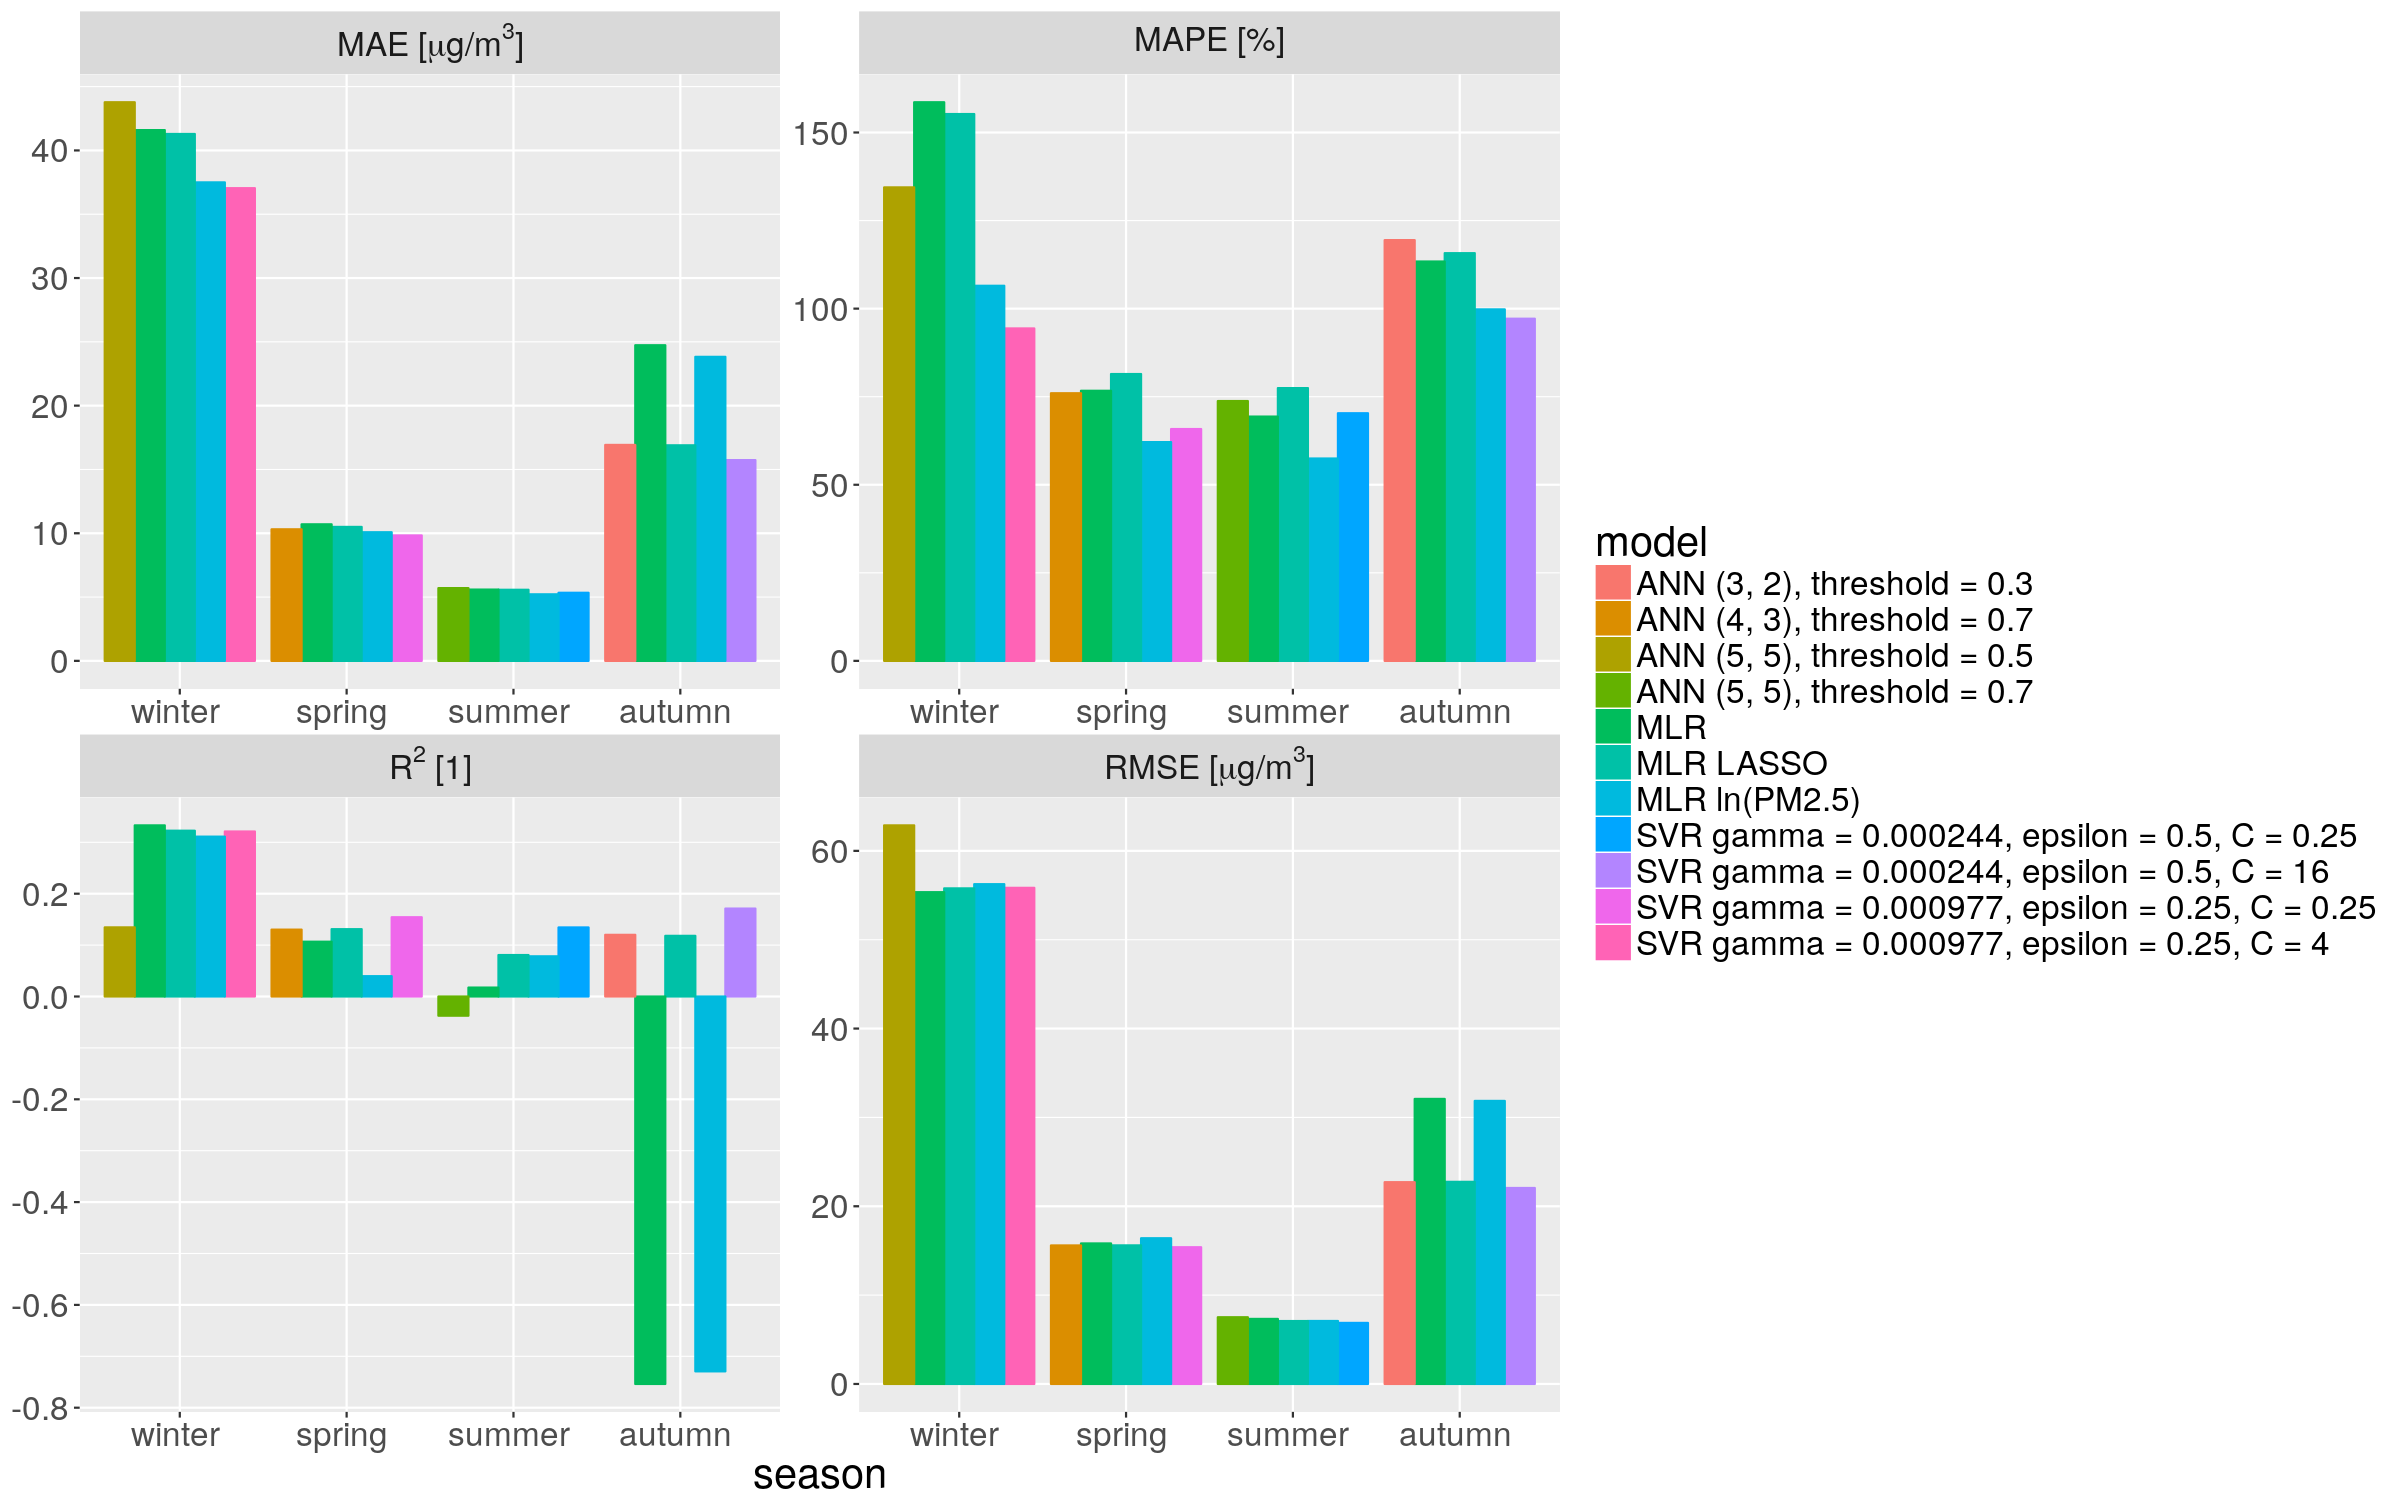
\includegraphics[width=\linewidth]{{figures/results/bujaka_same_season_plot}.png}
\caption{Results of the best models - GIOŚ Bujaka, all data }
\label{fig:results-best-bujaka-all-data}
\end{figure}
\end{landscape}

\begin{landscape}
\begin{figure}[htp]
\centering
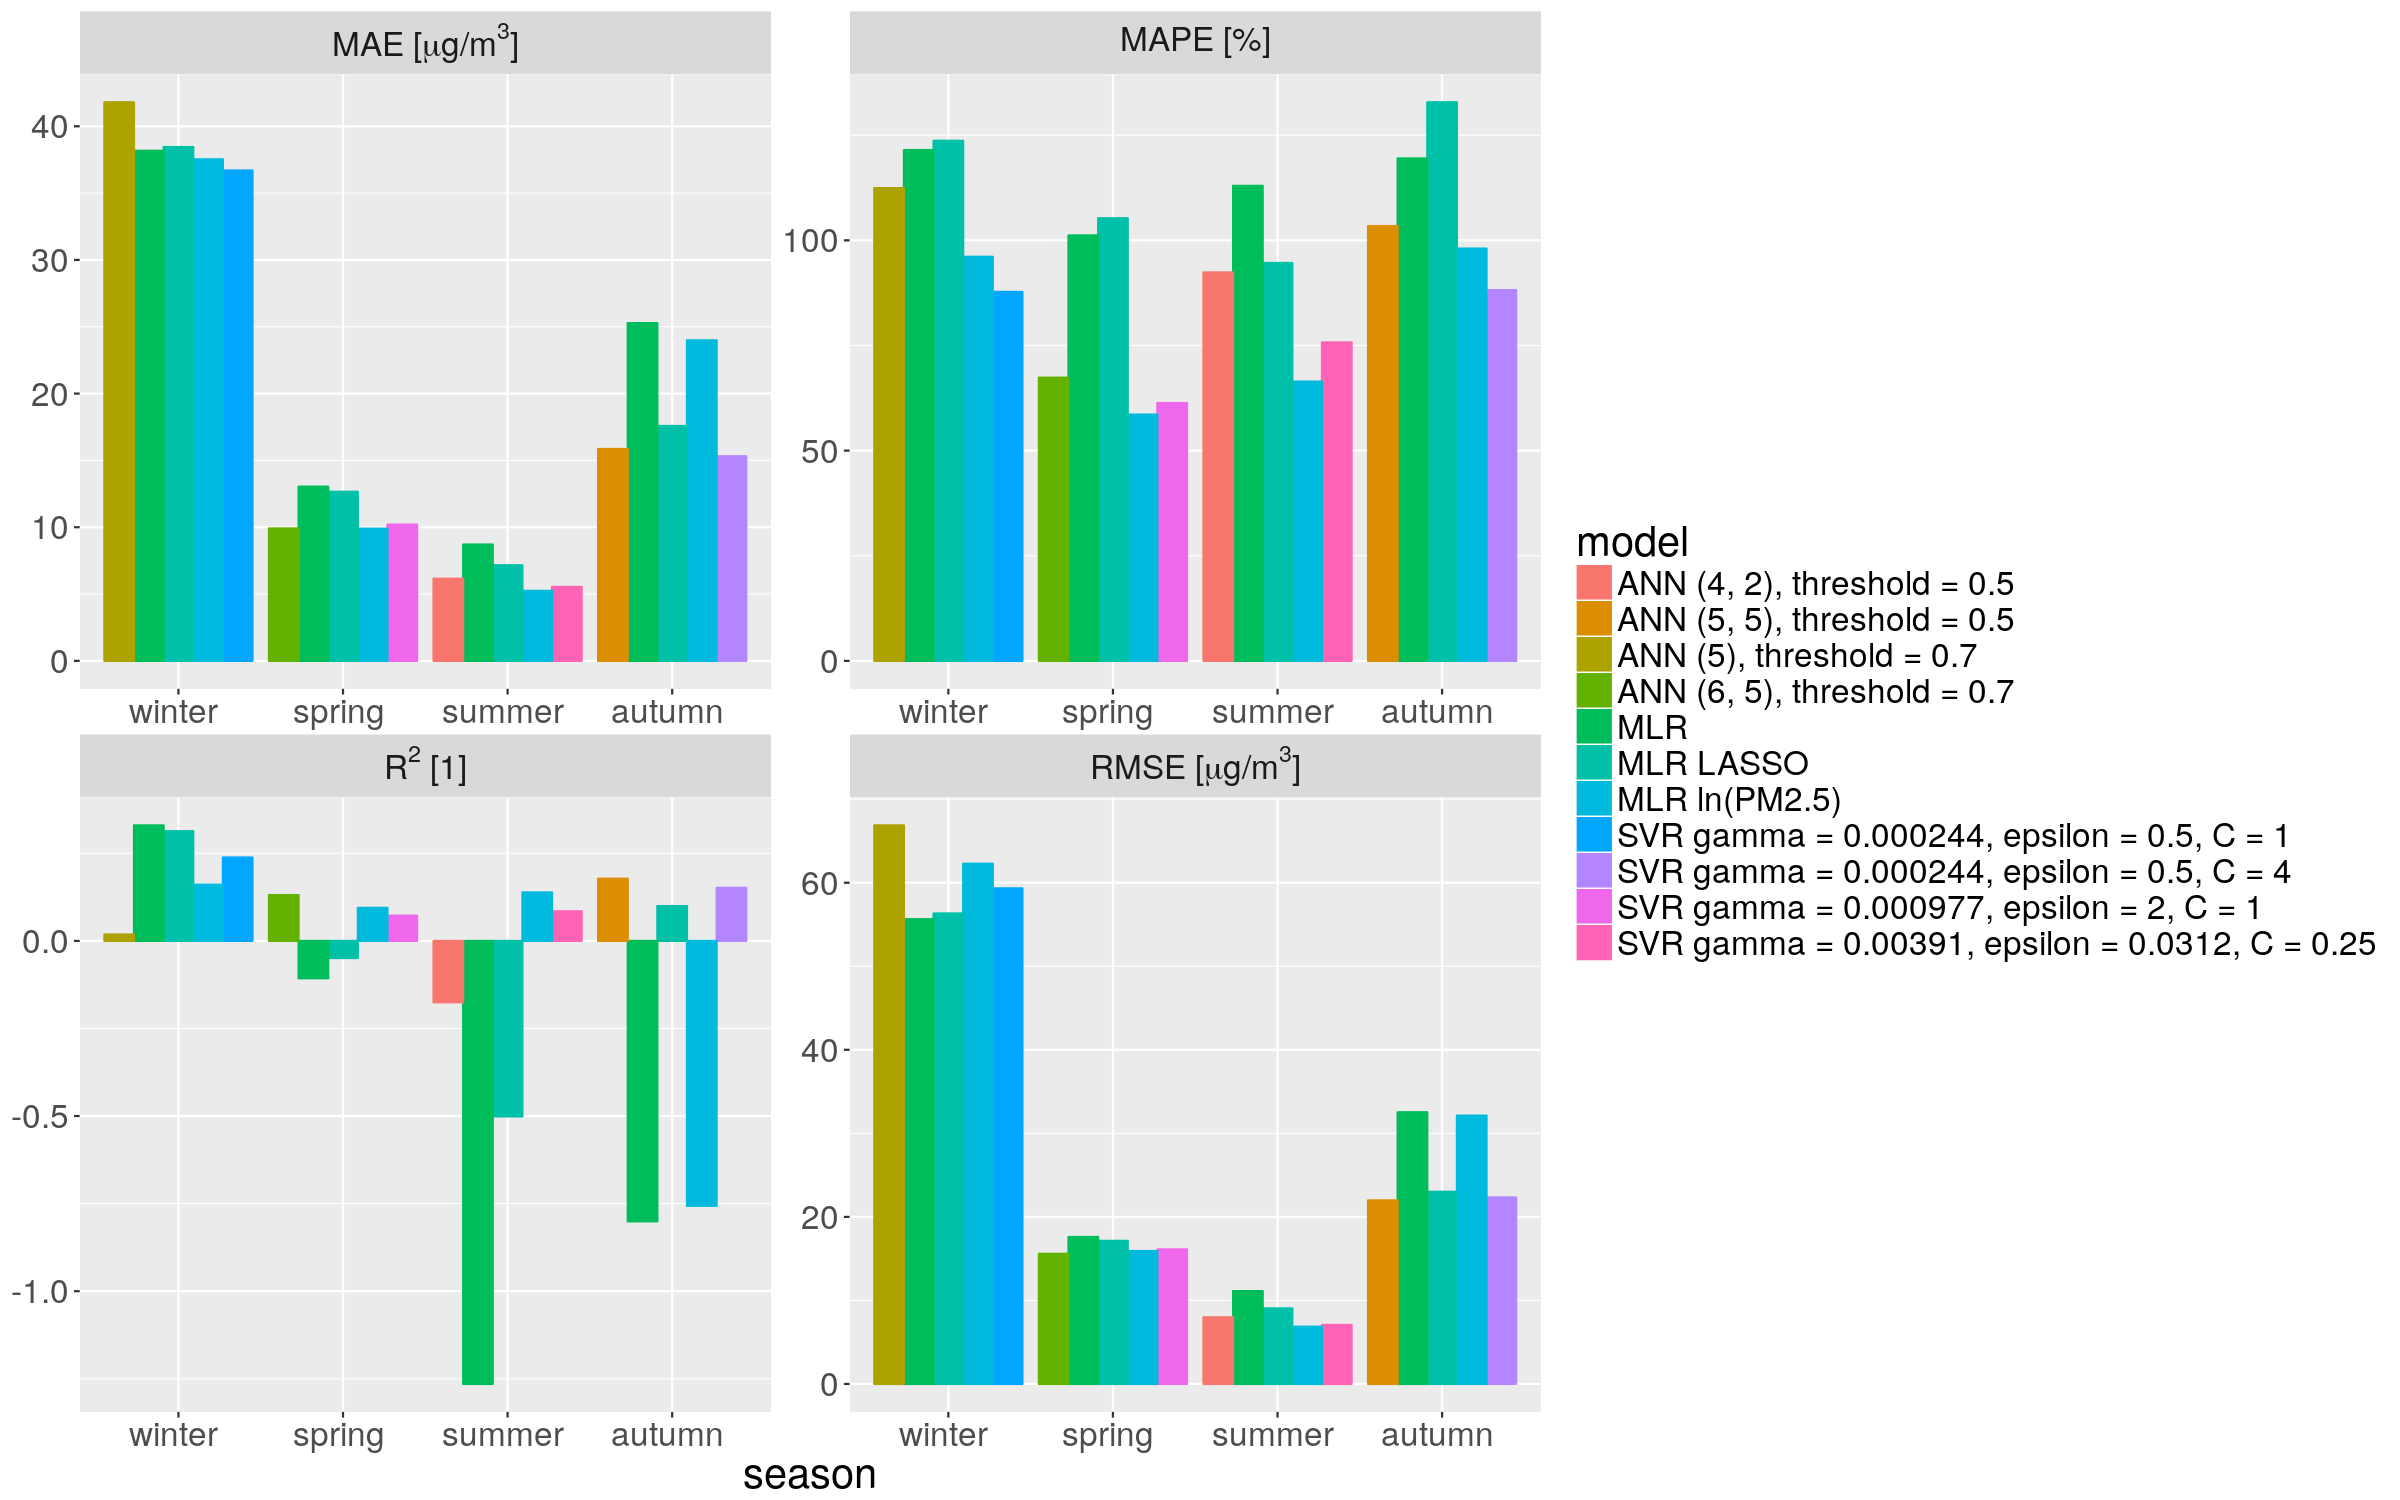
\includegraphics[width=\linewidth]{{figures/results/bujaka_continuous_plot}.png}
\caption{Results of the best models - GIOŚ Bujaka, same season }
\label{fig:results-best-bujaka-same-season}
\end{figure}
\end{landscape}

\begin{landscape}
\begin{figure}[htp]
\centering
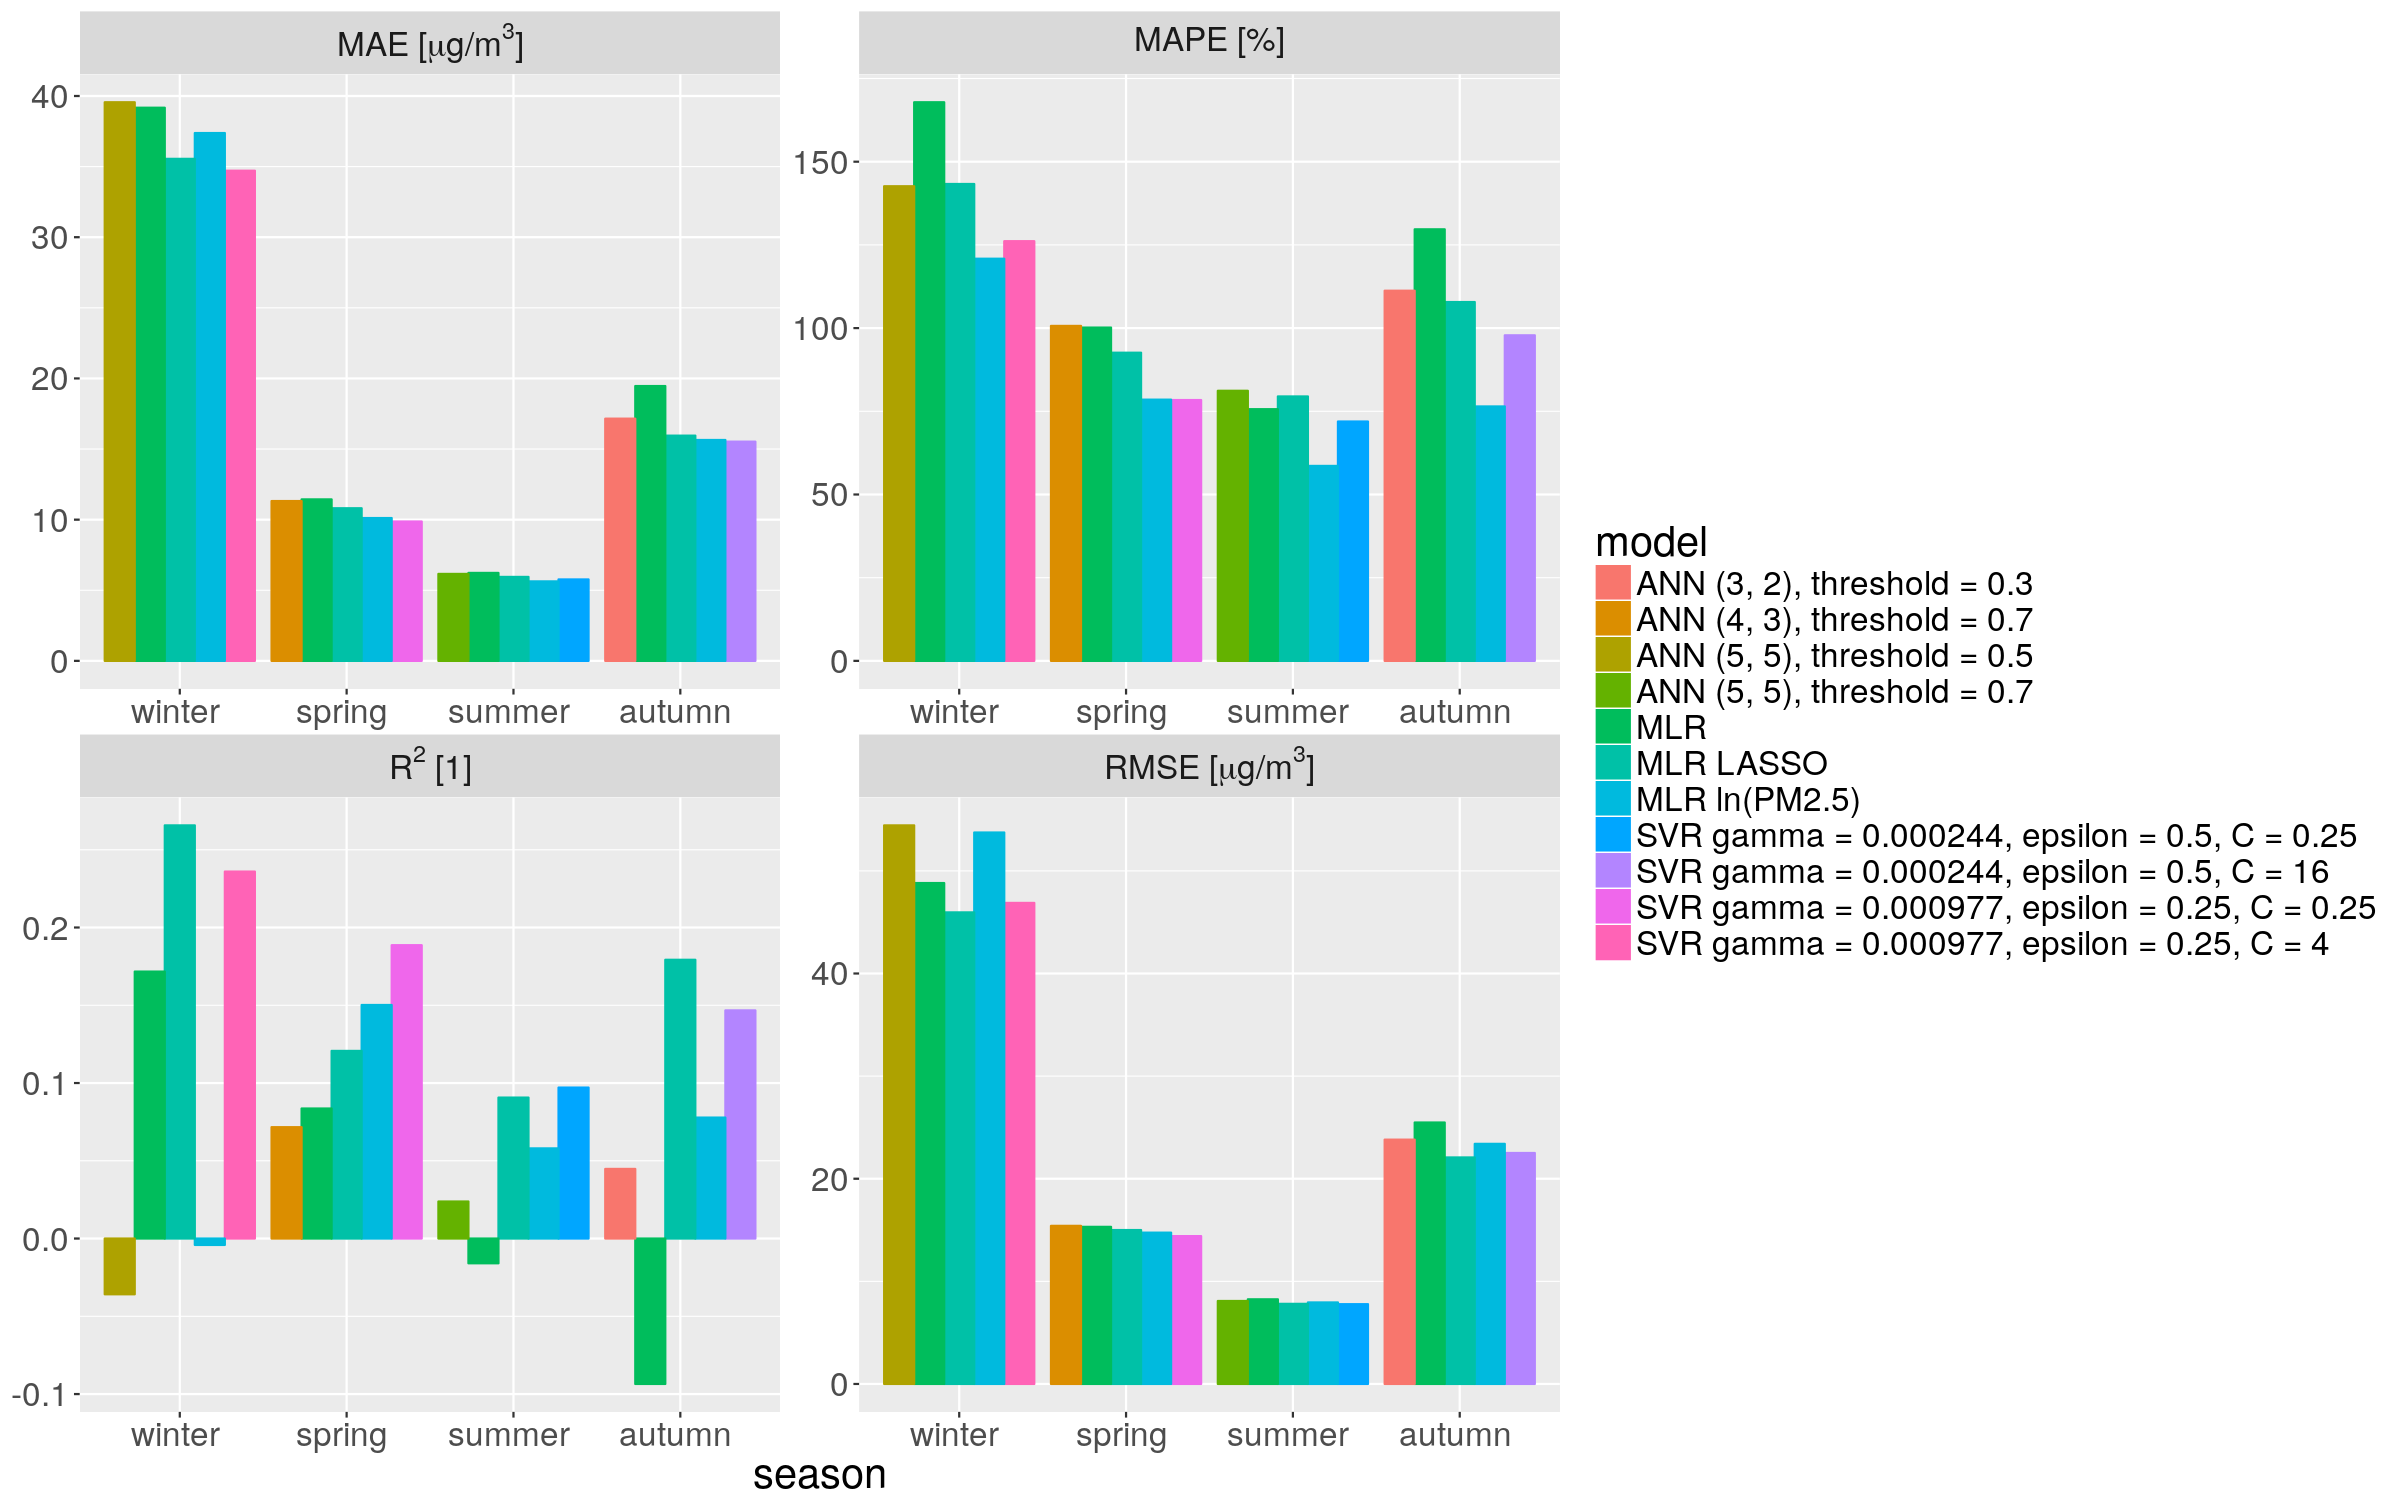
\includegraphics[width=\linewidth]{{figures/results/bulwarowa_same_season_plot}.png}
\caption{Results of the best models - GIOŚ Bulwarowa, all data }
\label{fig:results-best-bulwarowa-all-datat}
\end{figure}
\end{landscape}

\begin{landscape}
\begin{figure}[htp]
\centering
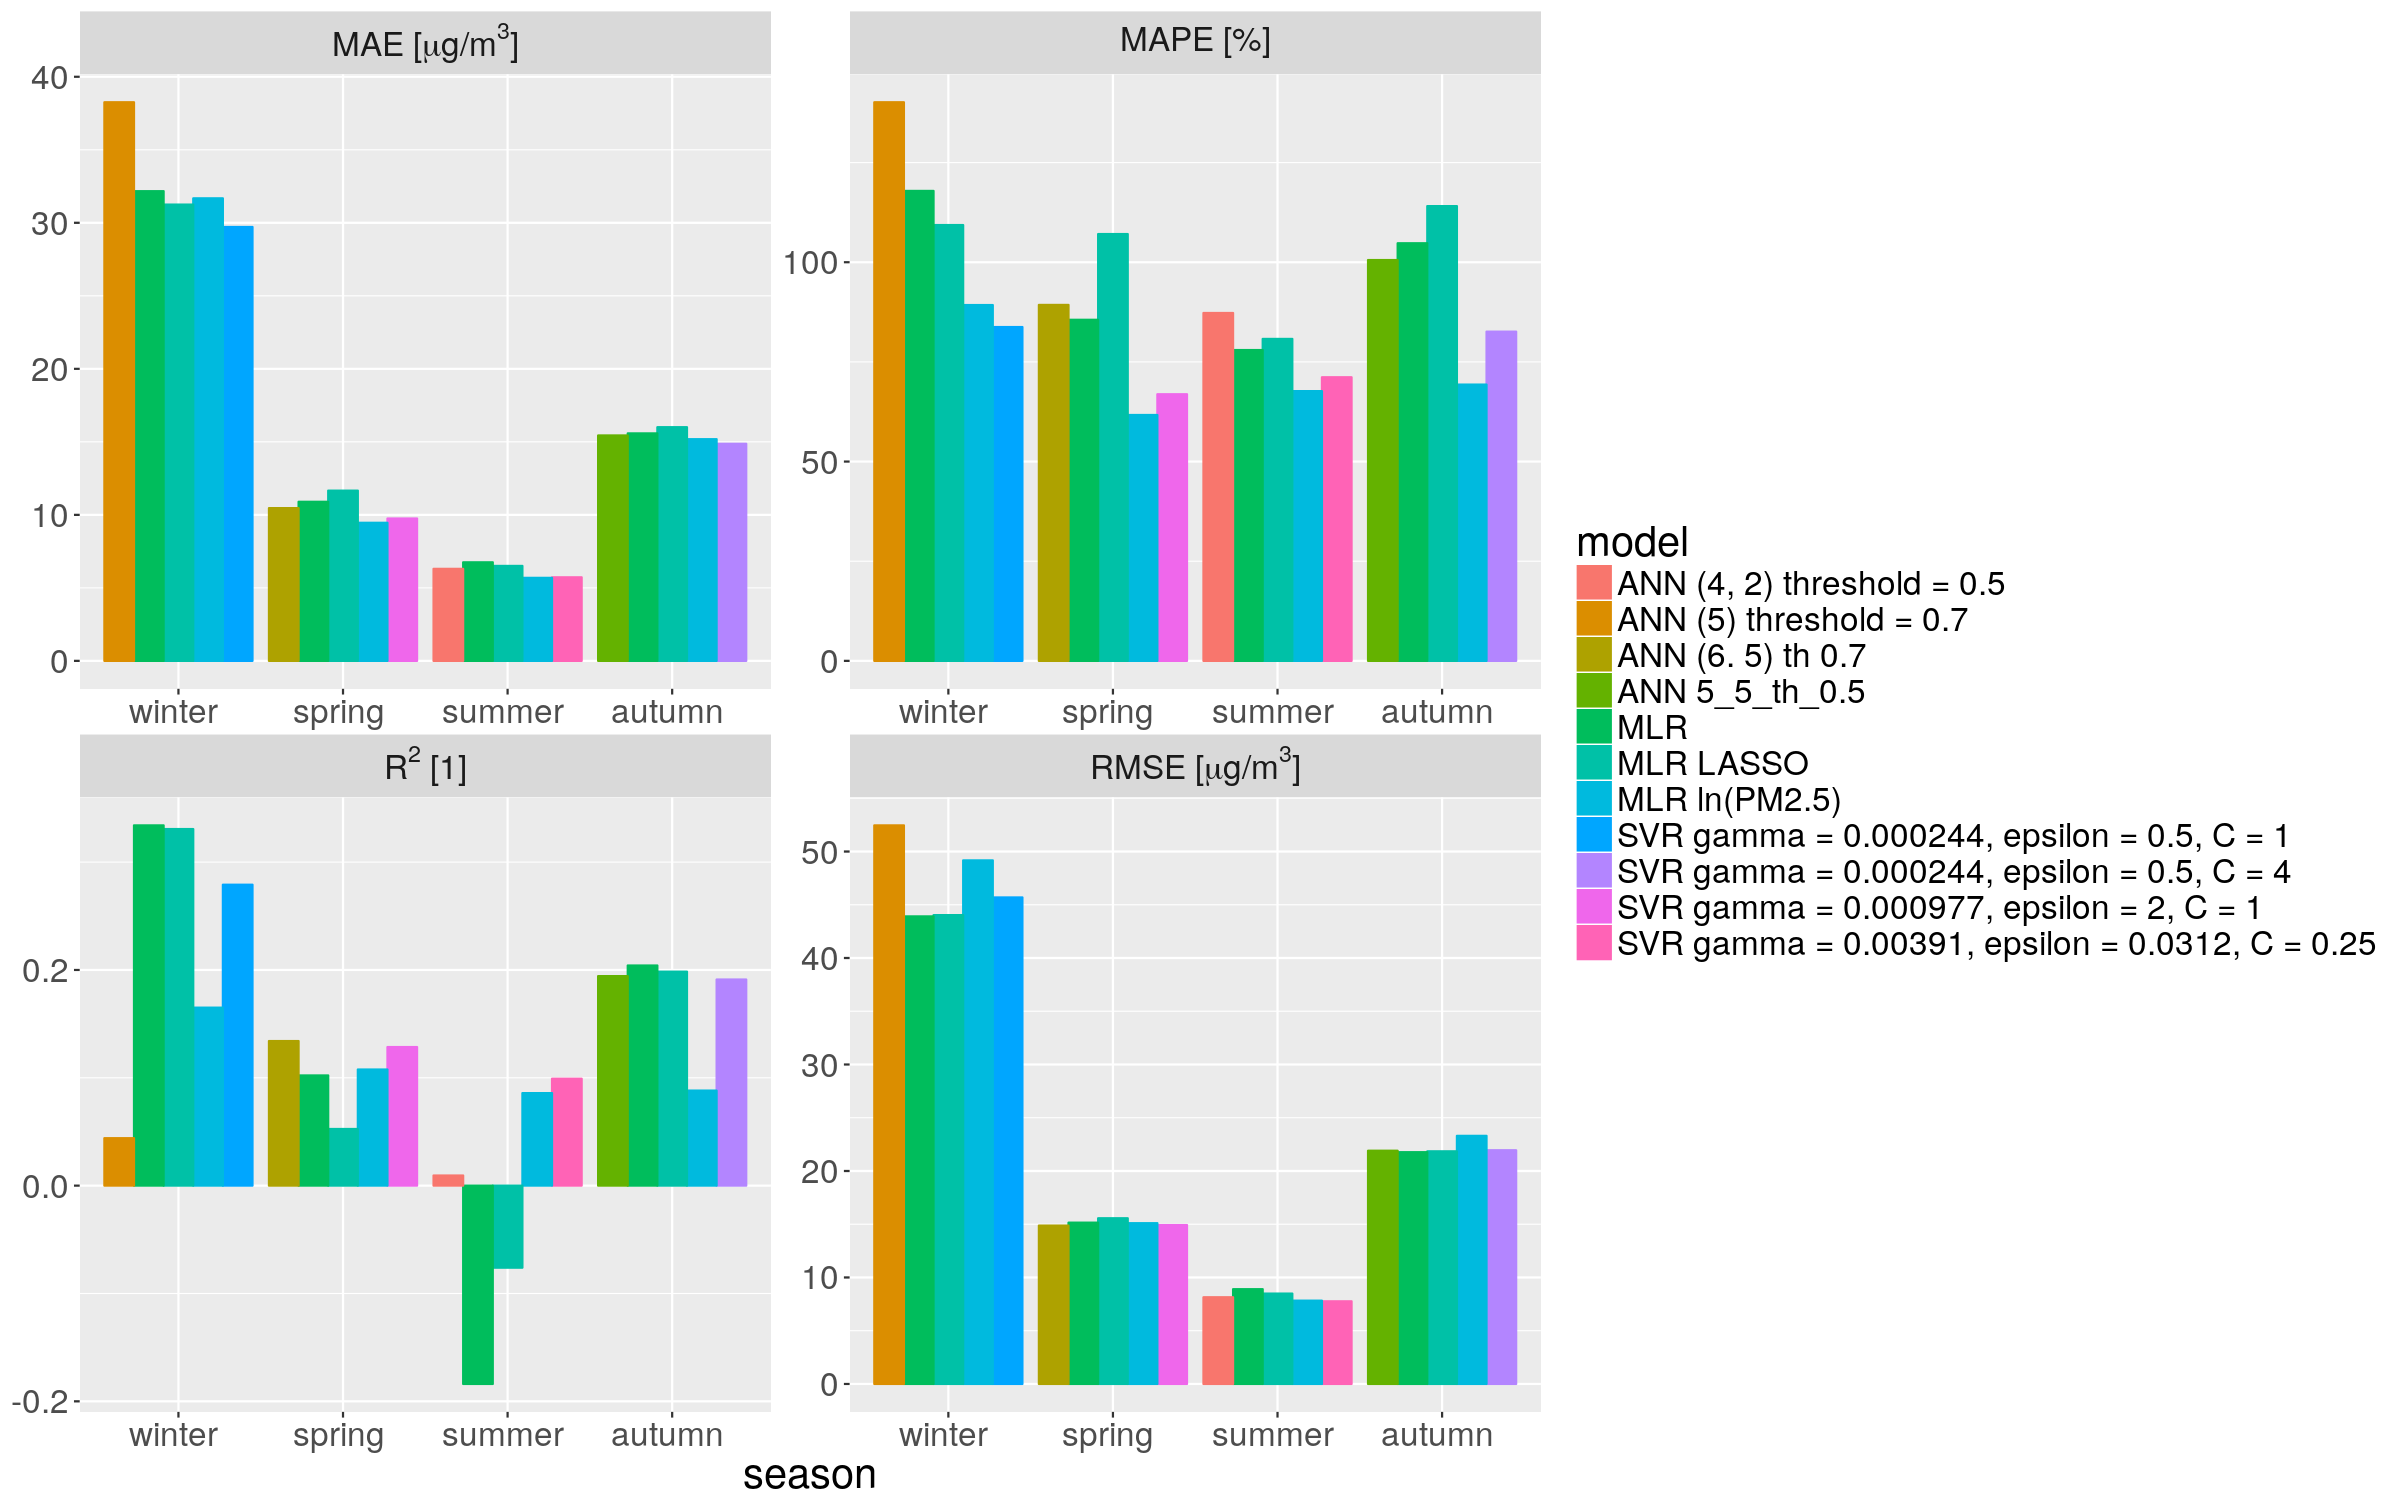
\includegraphics[width=\linewidth]{{figures/results/bulwarowa_continuous_plot}.png}
\caption{Results of the best models - GIOŚ Bulwarowa, same season }
\label{fig:results-best-bulwarowa-same-season}
\end{figure}
\end{landscape}

\begin{landscape}
\begin{figure}[htp]
\centering
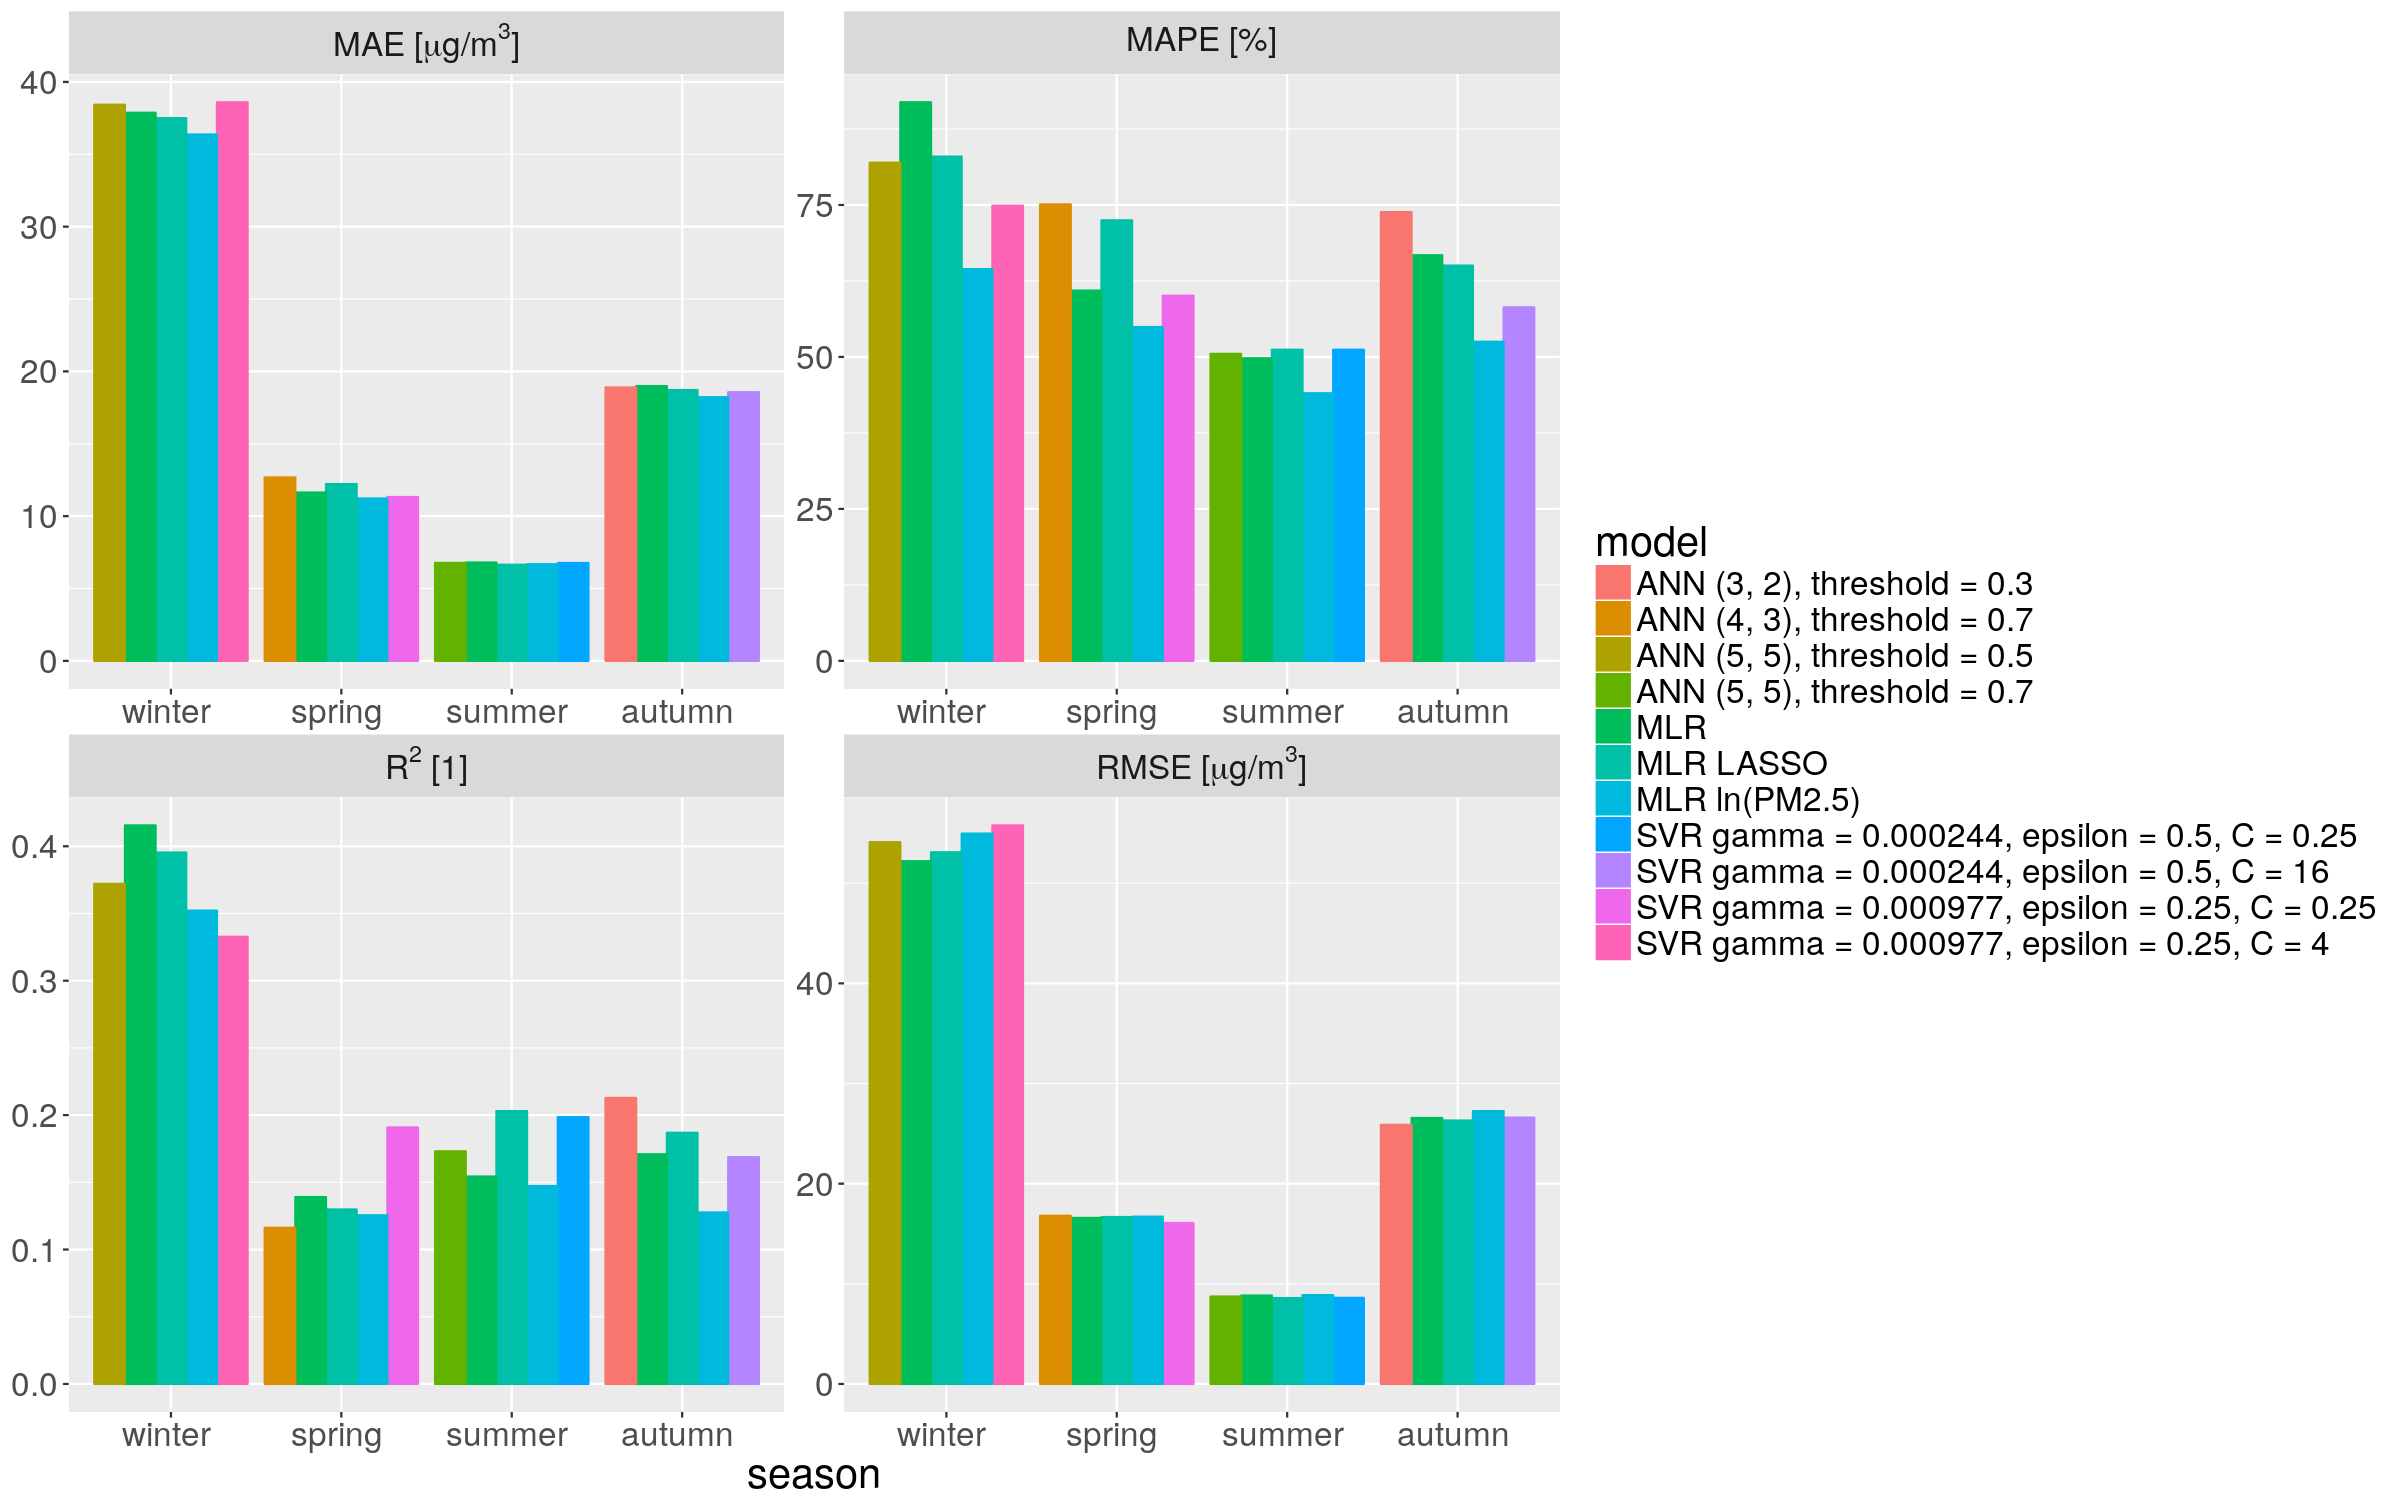
\includegraphics[width=\linewidth]{{figures/results/krasinskiego_same_season_plot}.png}
\caption{Results of the best models - GIOŚ Krasińskiego, all data }
\label{fig:results-best-krasinskiego-all-data}
\end{figure}
\end{landscape}

\begin{landscape}
\begin{figure}[htp]
\centering
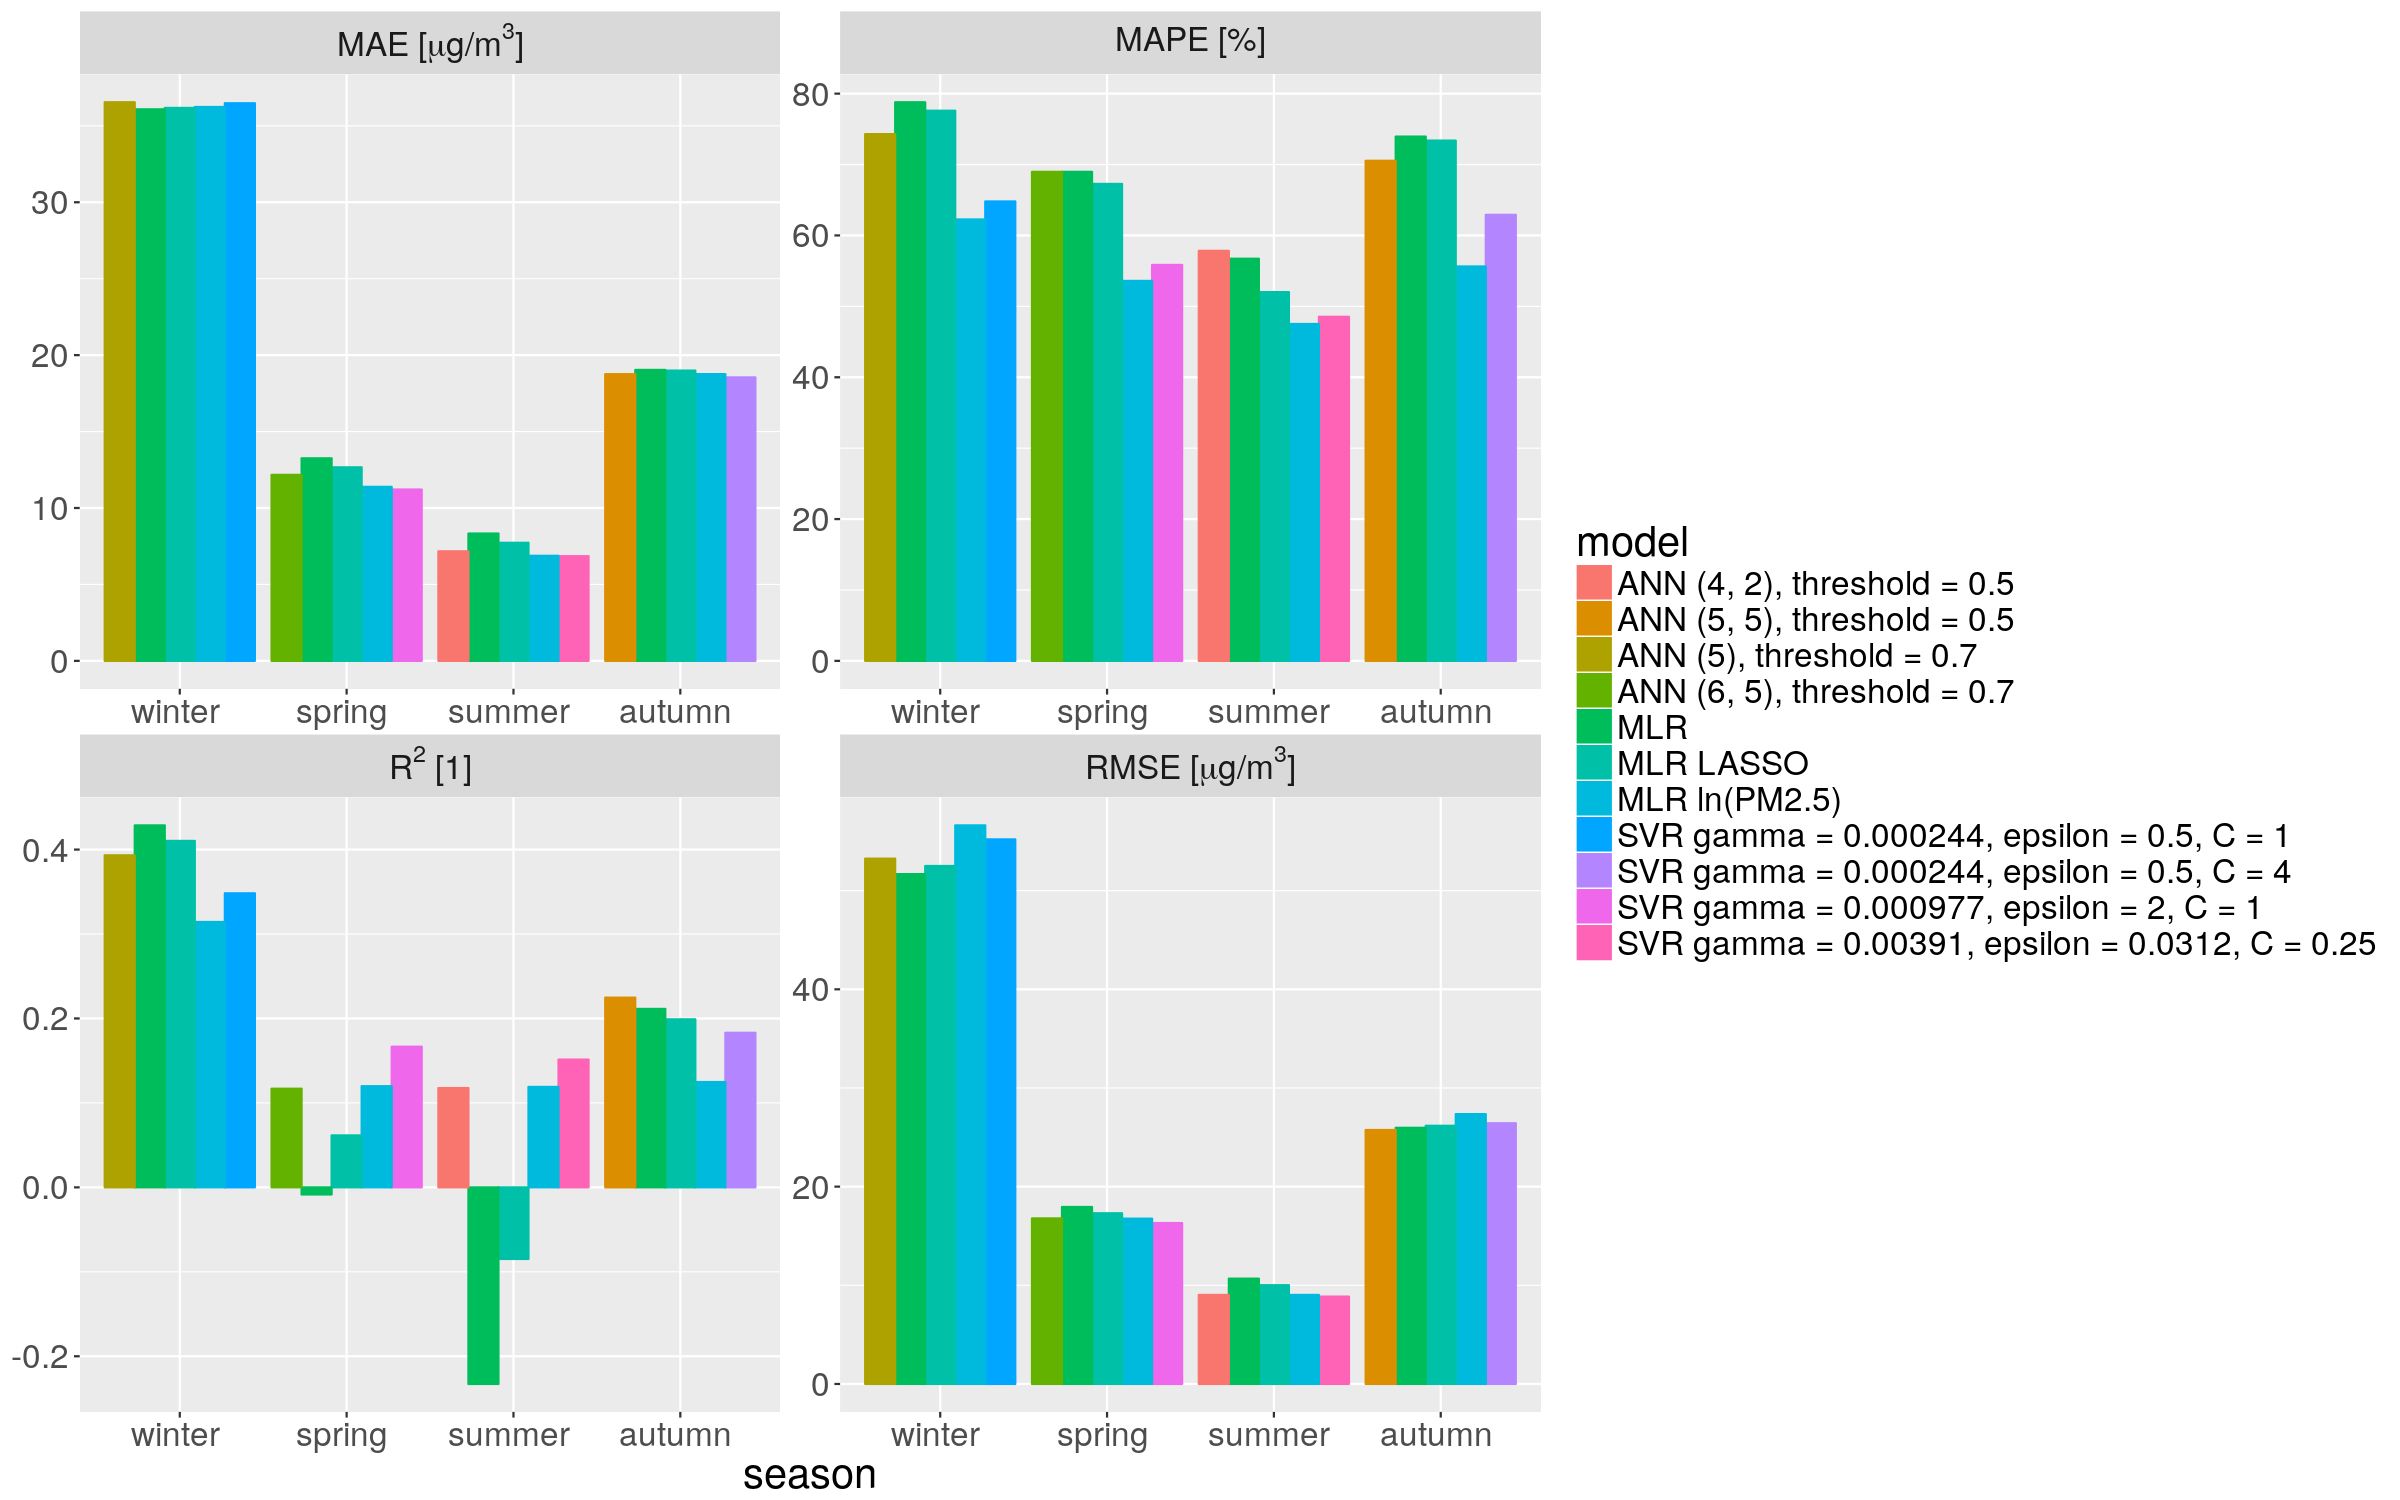
\includegraphics[width=\linewidth]{{figures/results/krasinskiego_continuous_plot}.png}
\caption{Results of the best models - GIOŚ Krasińskiego, same season }
\label{fig:results-best-krasinskiego-same-season}
\end{figure}
\end{landscape}

% comparison of actual and predicted PM2.5 concentrations
% GIOŚ Bujaka

% \begin{landscape}
% \begin{figure}[htp]
% \centering
% \includegraphics[width=\linewidth]{{figures/results/best-models/bujaka/all-data/winter/comparison_plot_mlr_lag_24}.png}
% \caption{Comparison of actual and predicted PM2.5 concentrations - GIOŚ Bujaka, winter, all data }
% \label{fig:results-comparison-bujaka-winter-all-data}
% \end{figure}
% \end{landscape}

% \begin{landscape}
% \begin{figure}[htp]
% \centering
% \includegraphics[width=\linewidth]{{figures/results/best-models/bujaka/same-season/winter/all_comparison_plot_mlr_lag_24}.png}
% \caption{Comparison of actual and predicted PM2.5 concentrations - GIOŚ Bujaka, winter, same season }
% \label{fig:results-comparison-bujaka-winter-same-season}
% \end{figure}
% \end{landscape}

% \begin{landscape}
% \begin{figure}[htp]
% \centering
% 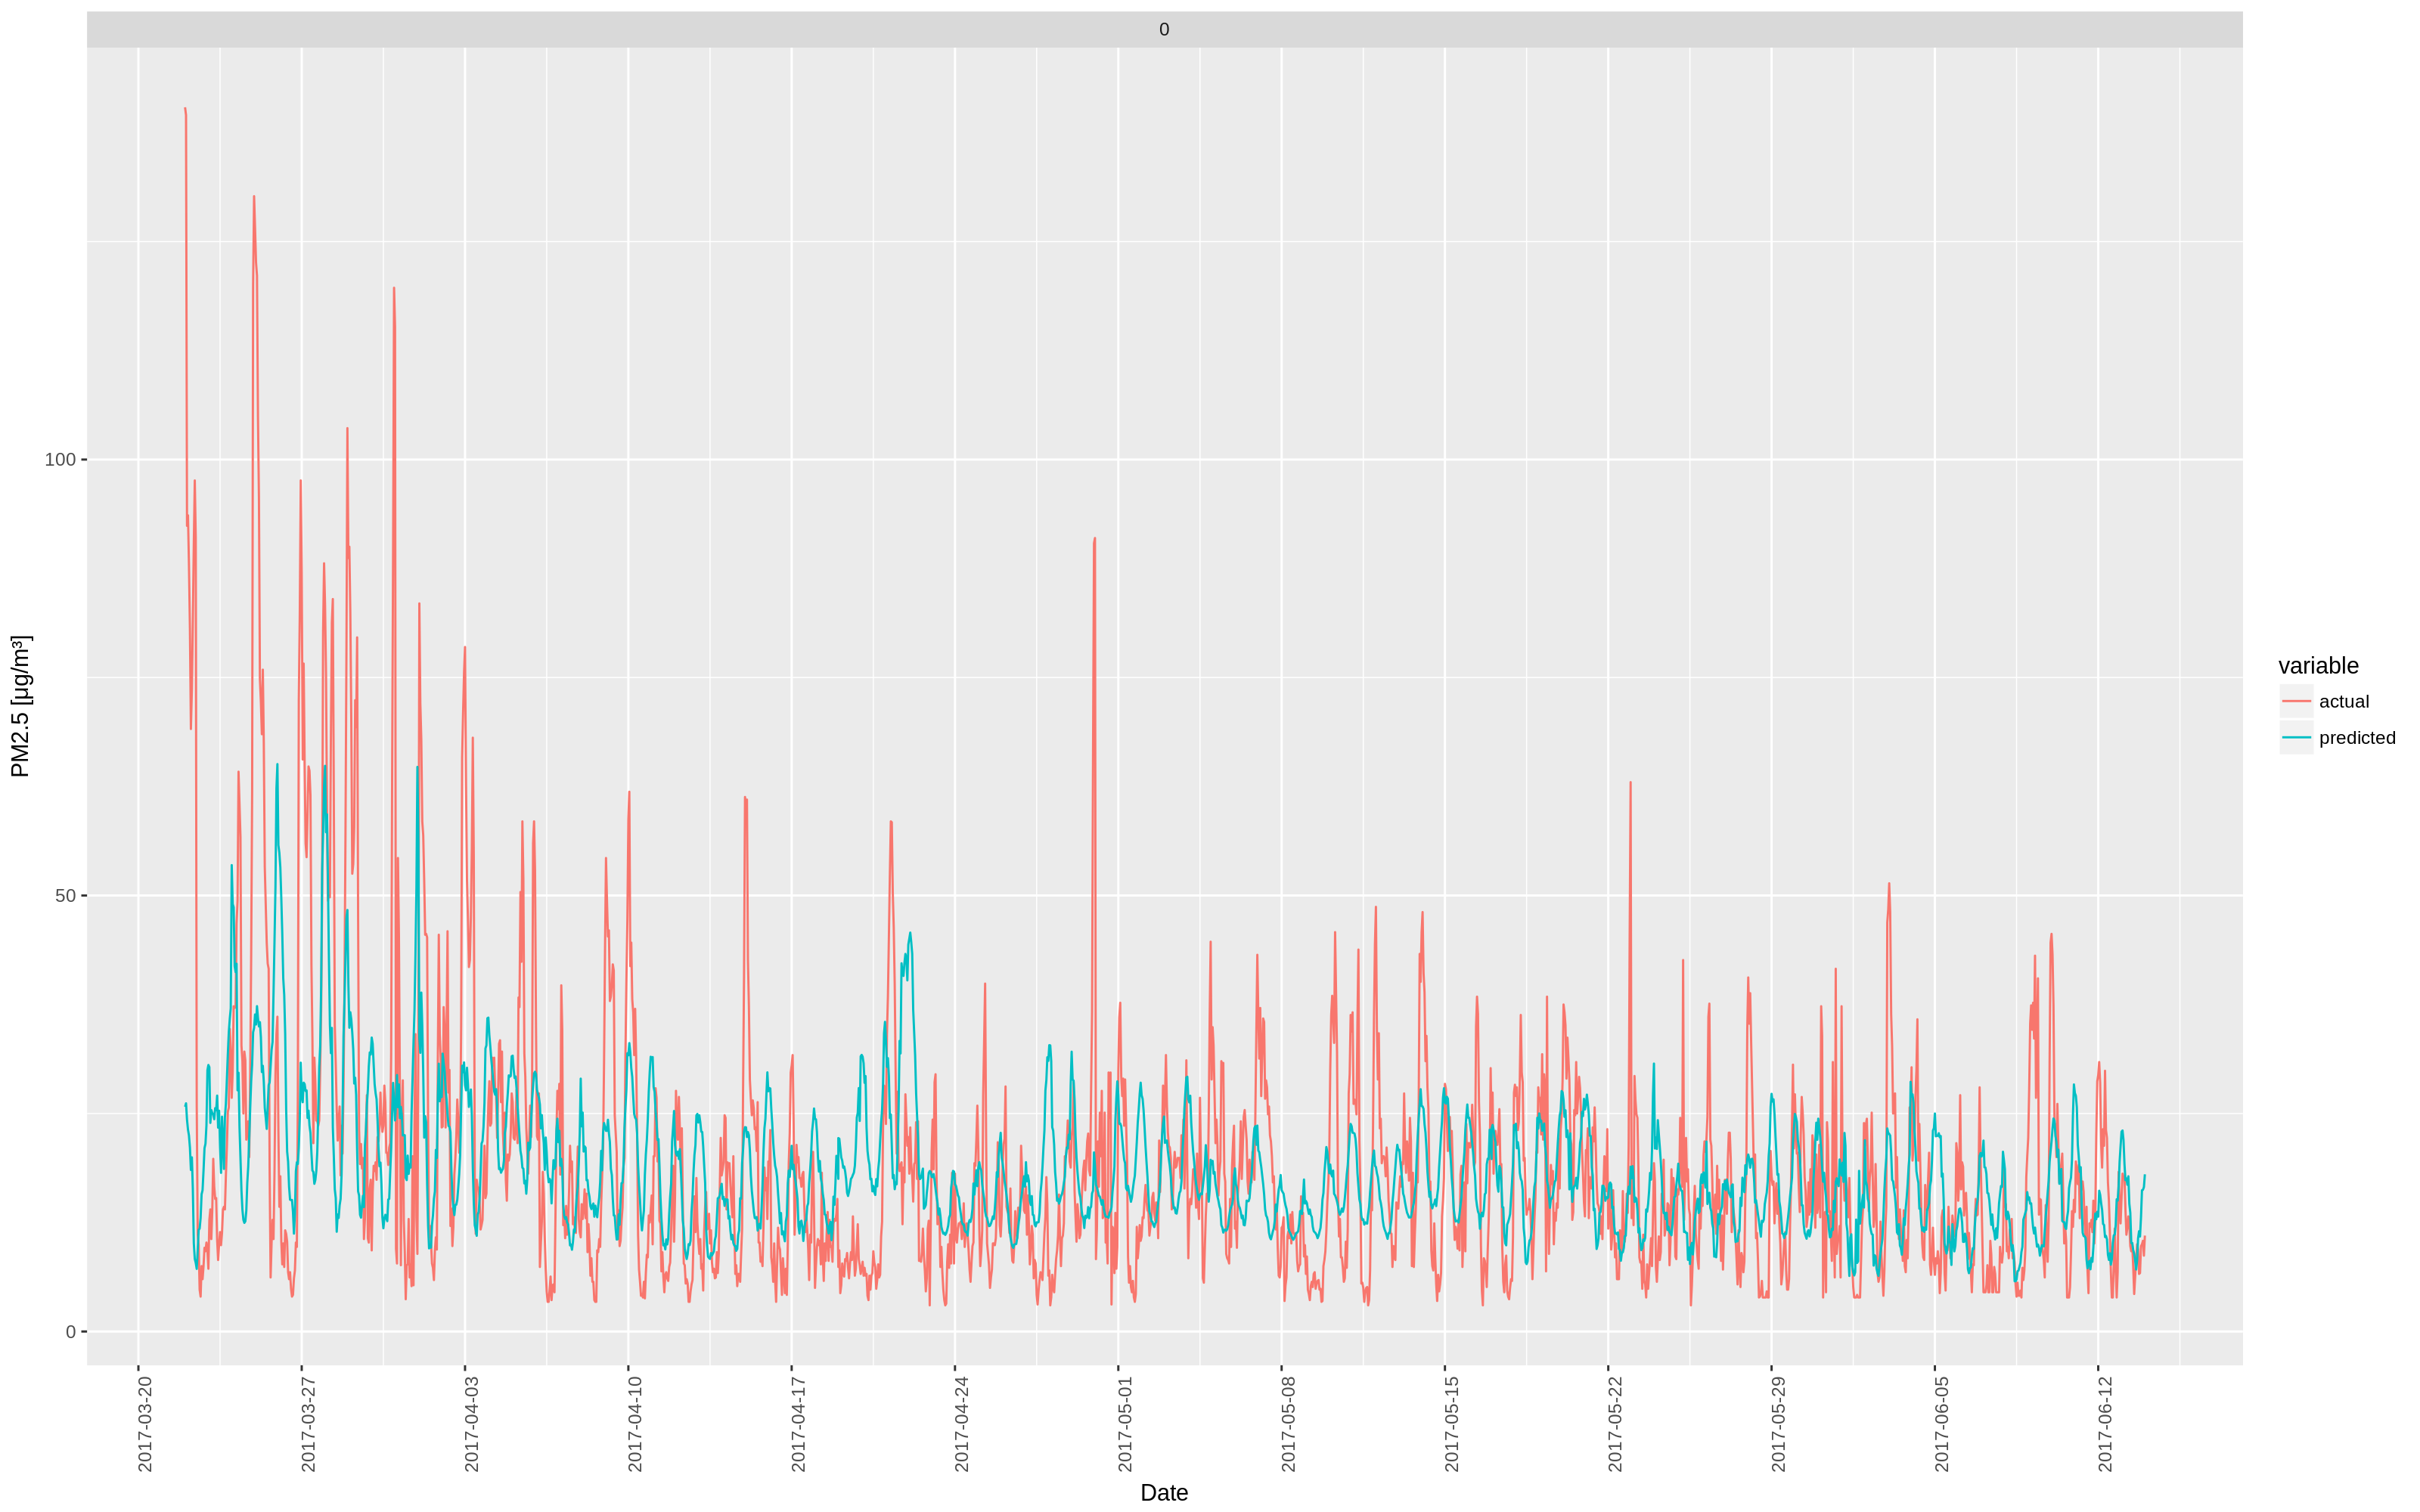
\includegraphics[width=\linewidth]{{figures/results/best-models/bujaka/all-data/spring/comparison_plot_mlp1_6_5_th_9.7_lag_24}.png}
% \caption{Comparison of actual and predicted PM2.5 concentrations - GIOŚ Bujaka, spring, all data }
% \label{fig:results-comparison-bujaka-spring-all-data}
% \end{figure}
% \end{landscape}

% \begin{landscape}
% \begin{figure}[htp]
% \centering
% \includegraphics[width=\linewidth]{{figures/results/best-models/bujaka/same-season/spring/all_comparison_plot_svr_gam0.000977_eps0.25_c0.25_lag_24}.png}
% \caption{Comparison of actual and predicted PM2.5 concentrations - GIOŚ Bujaka, spring, same season }
% \label{fig:results-comparison-bujaka-spring-same-season}
% \end{figure}
% \end{landscape}

% \begin{landscape}
% \begin{figure}[htp]
% \centering
% 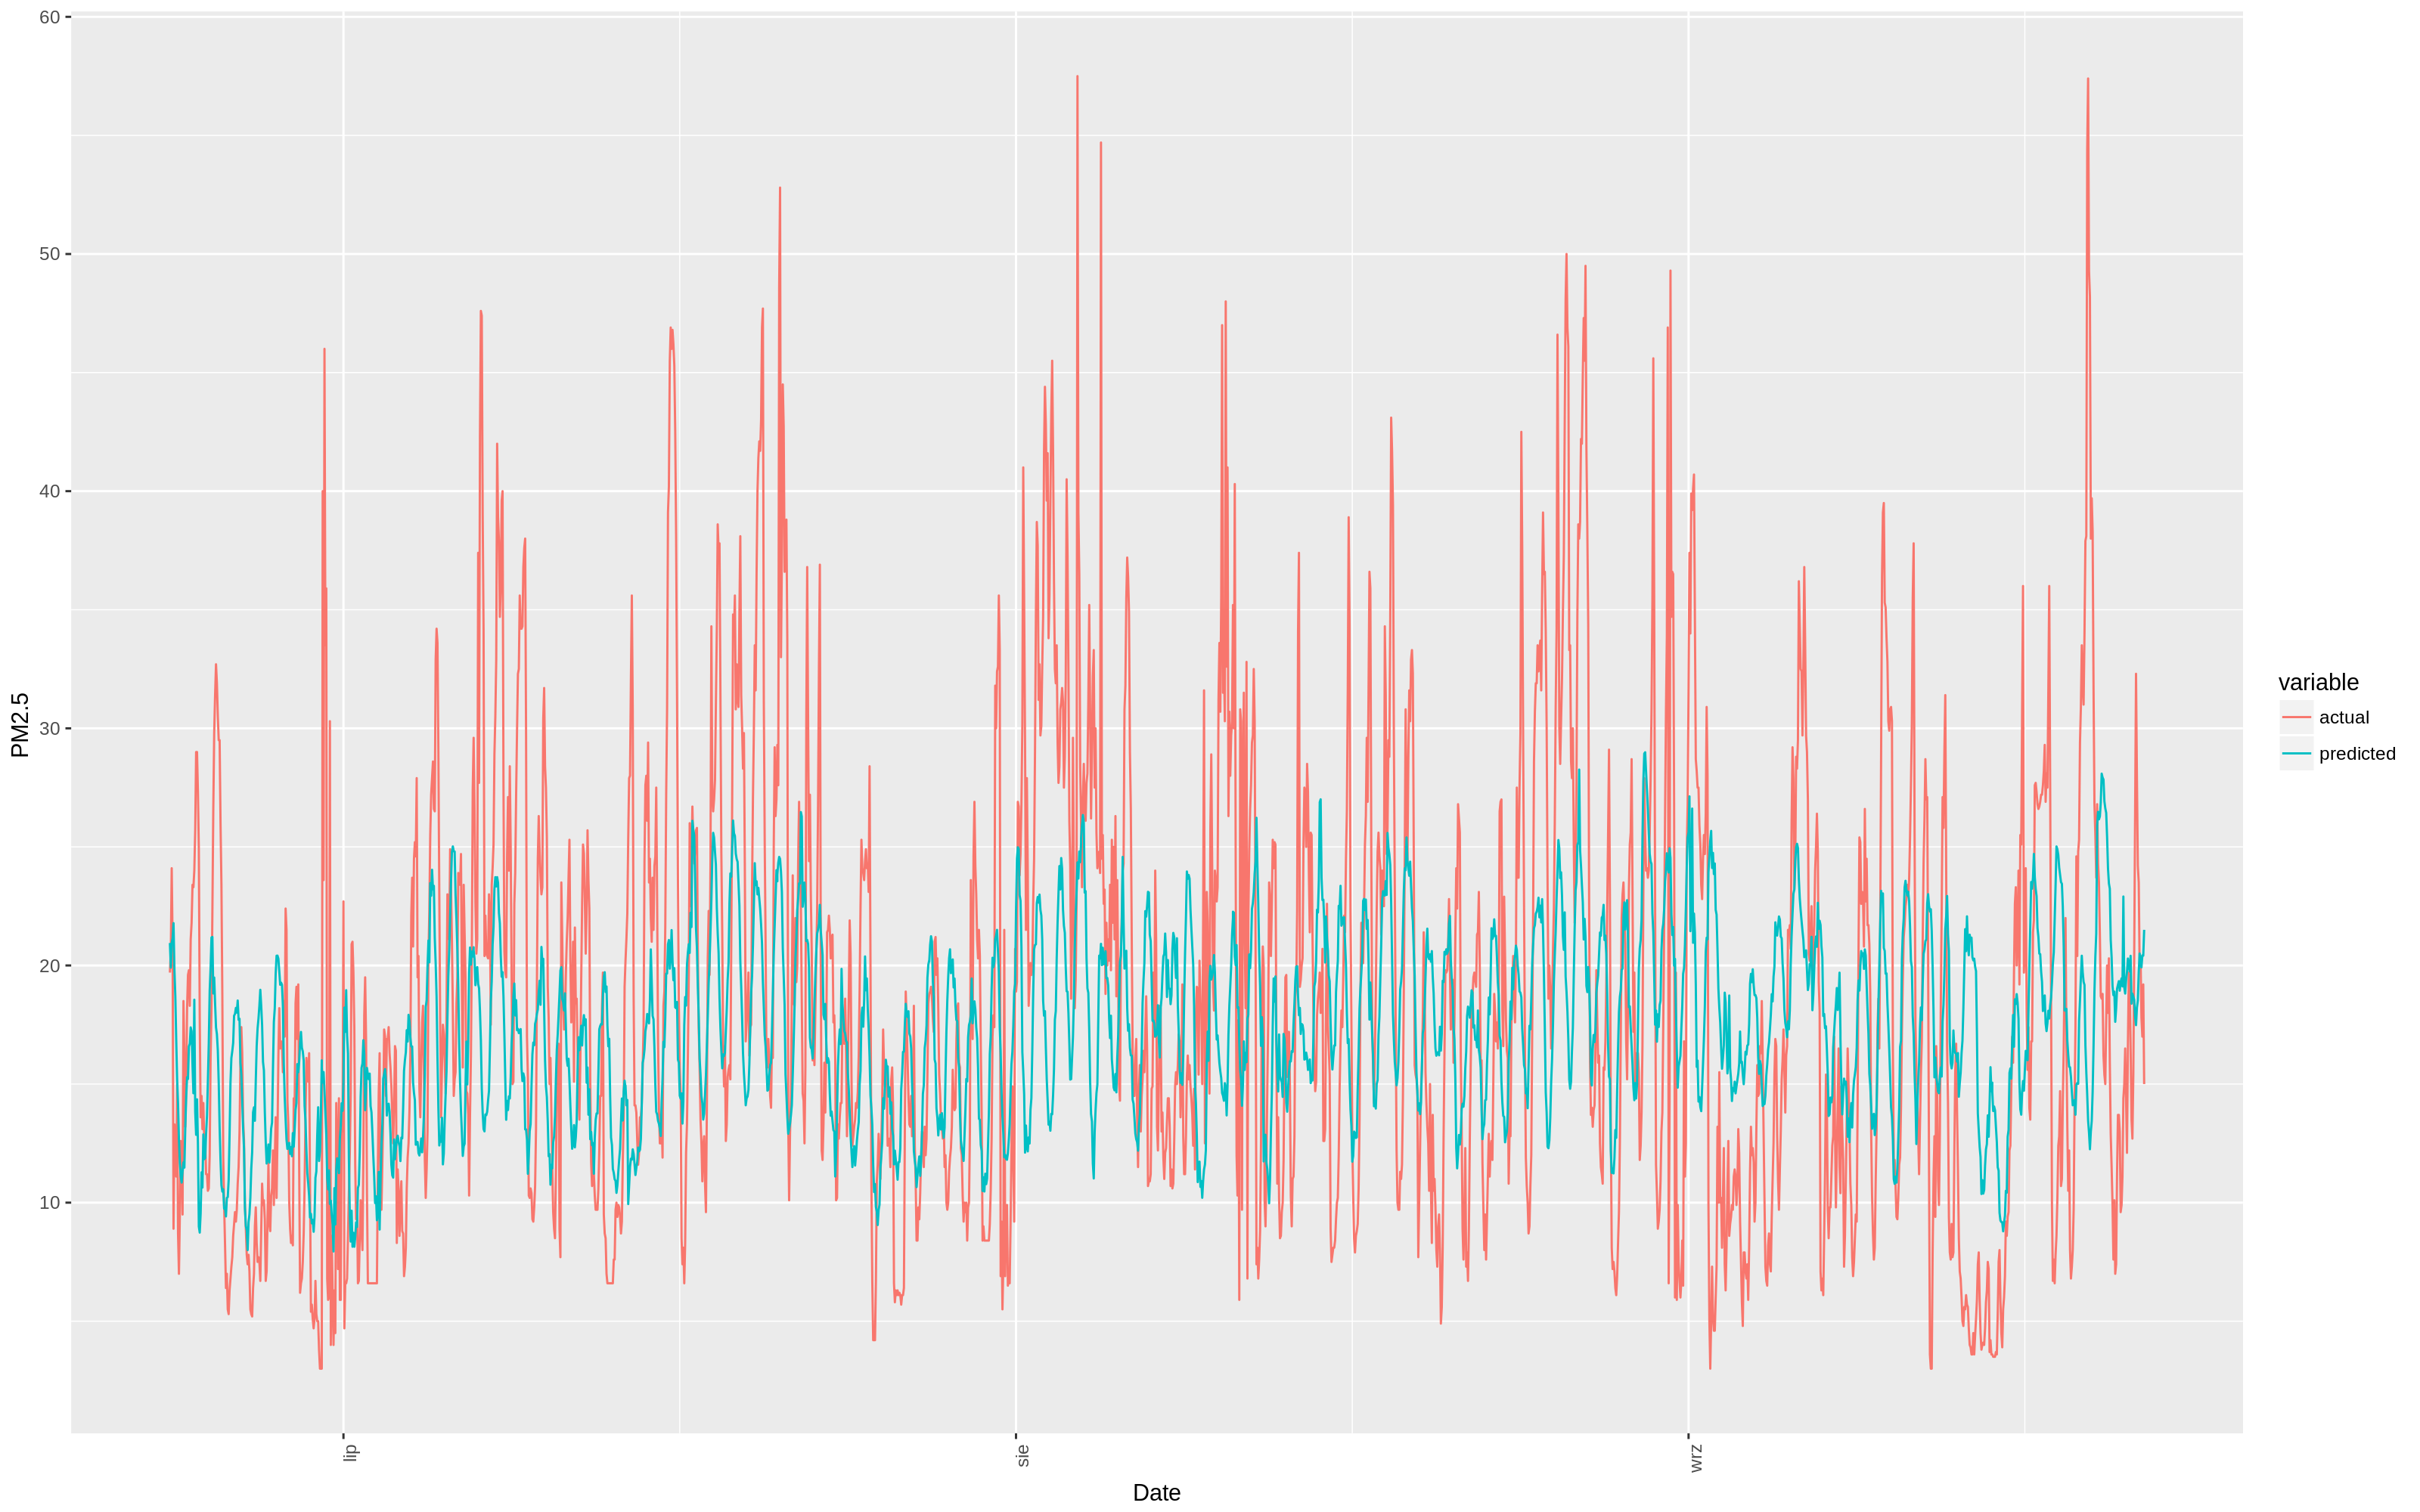
\includegraphics[width=\linewidth]{{figures/results/best-models/bujaka/all-data/summer/comparison_plot_log_mlr_lag_24}.png}
% \caption{Comparison of actual and predicted PM2.5 concentrations - GIOŚ Bujaka, summer, all data }
% \label{fig:results-comparison-bujaka-summer-all-data}
% \end{figure}
% \end{landscape}

% \begin{landscape}
% \begin{figure}[htp]
% \centering
% 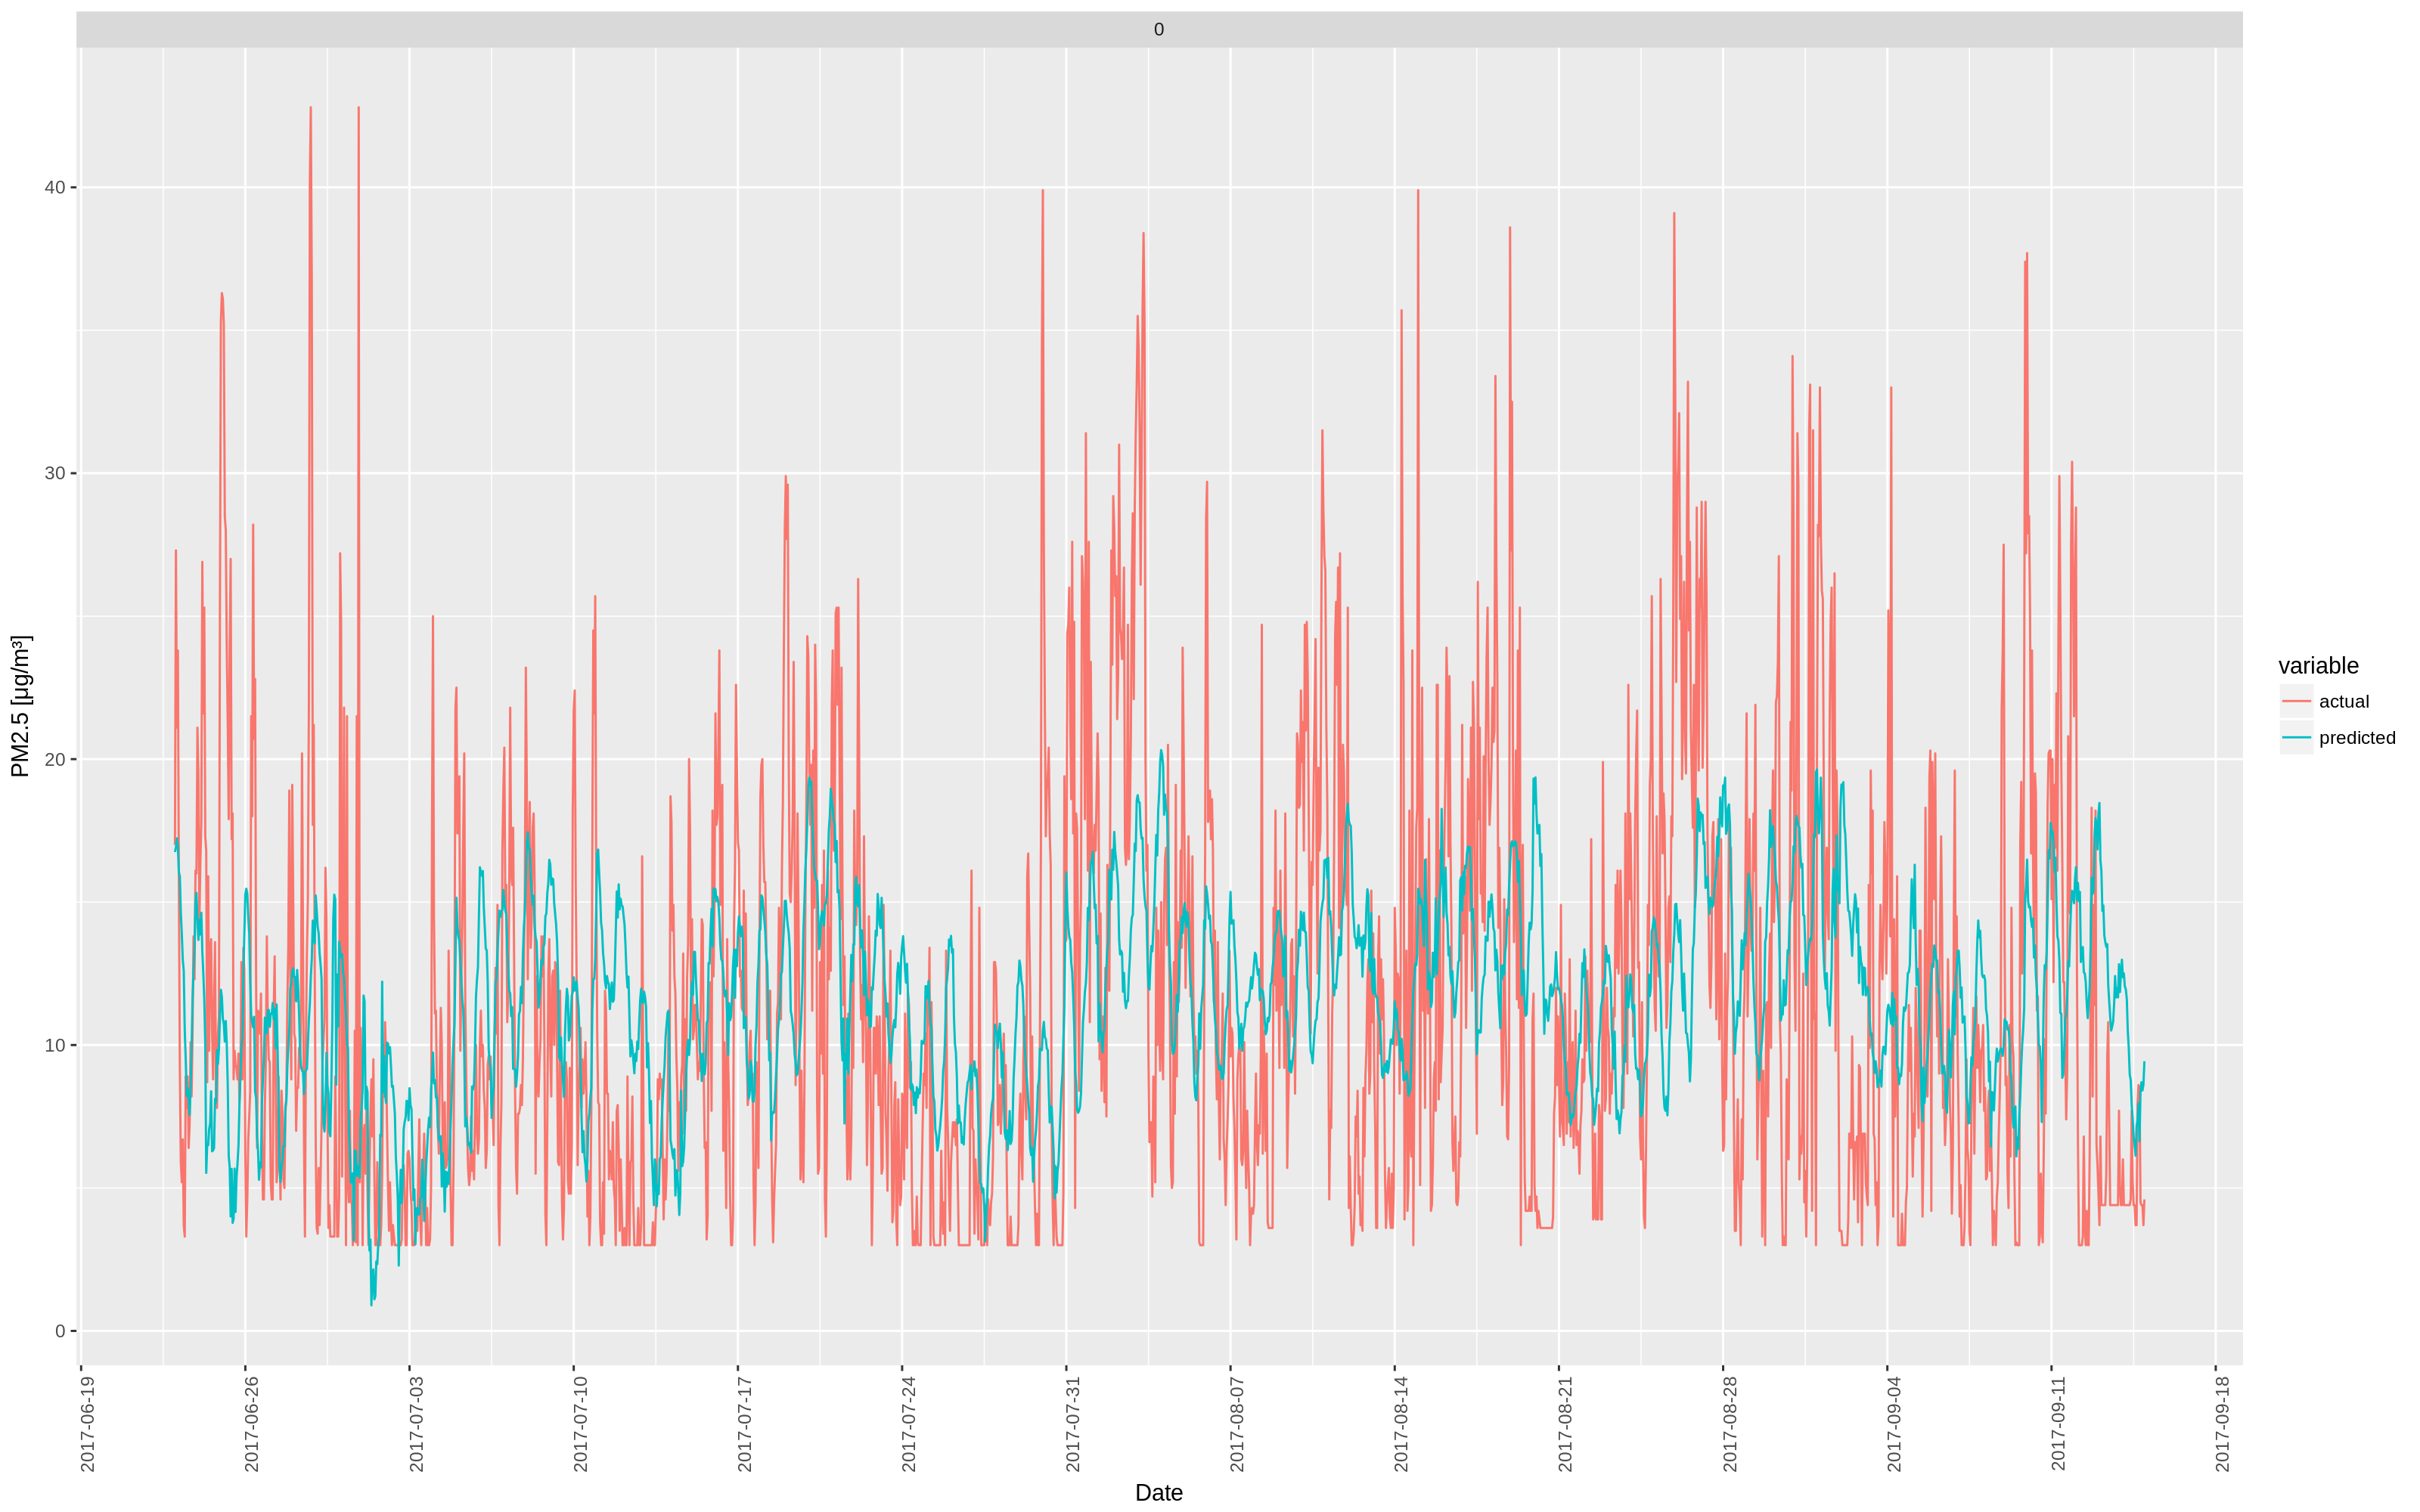
\includegraphics[width=\linewidth]{{figures/results/best-models/bujaka/same-season/summer/all_comparison_plot_svr_gam0.000244_eps0.5_c0.25_lag_24}.png}
% \caption{Comparison of actual and predicted PM2.5 concentrations - GIOŚ Bujaka, spring, same season }
% \label{fig:results-comparison-bujaka-summer-same-season}
% \end{figure}
% \end{landscape}

% \begin{landscape}
% \begin{figure}[htp]
% \centering
% 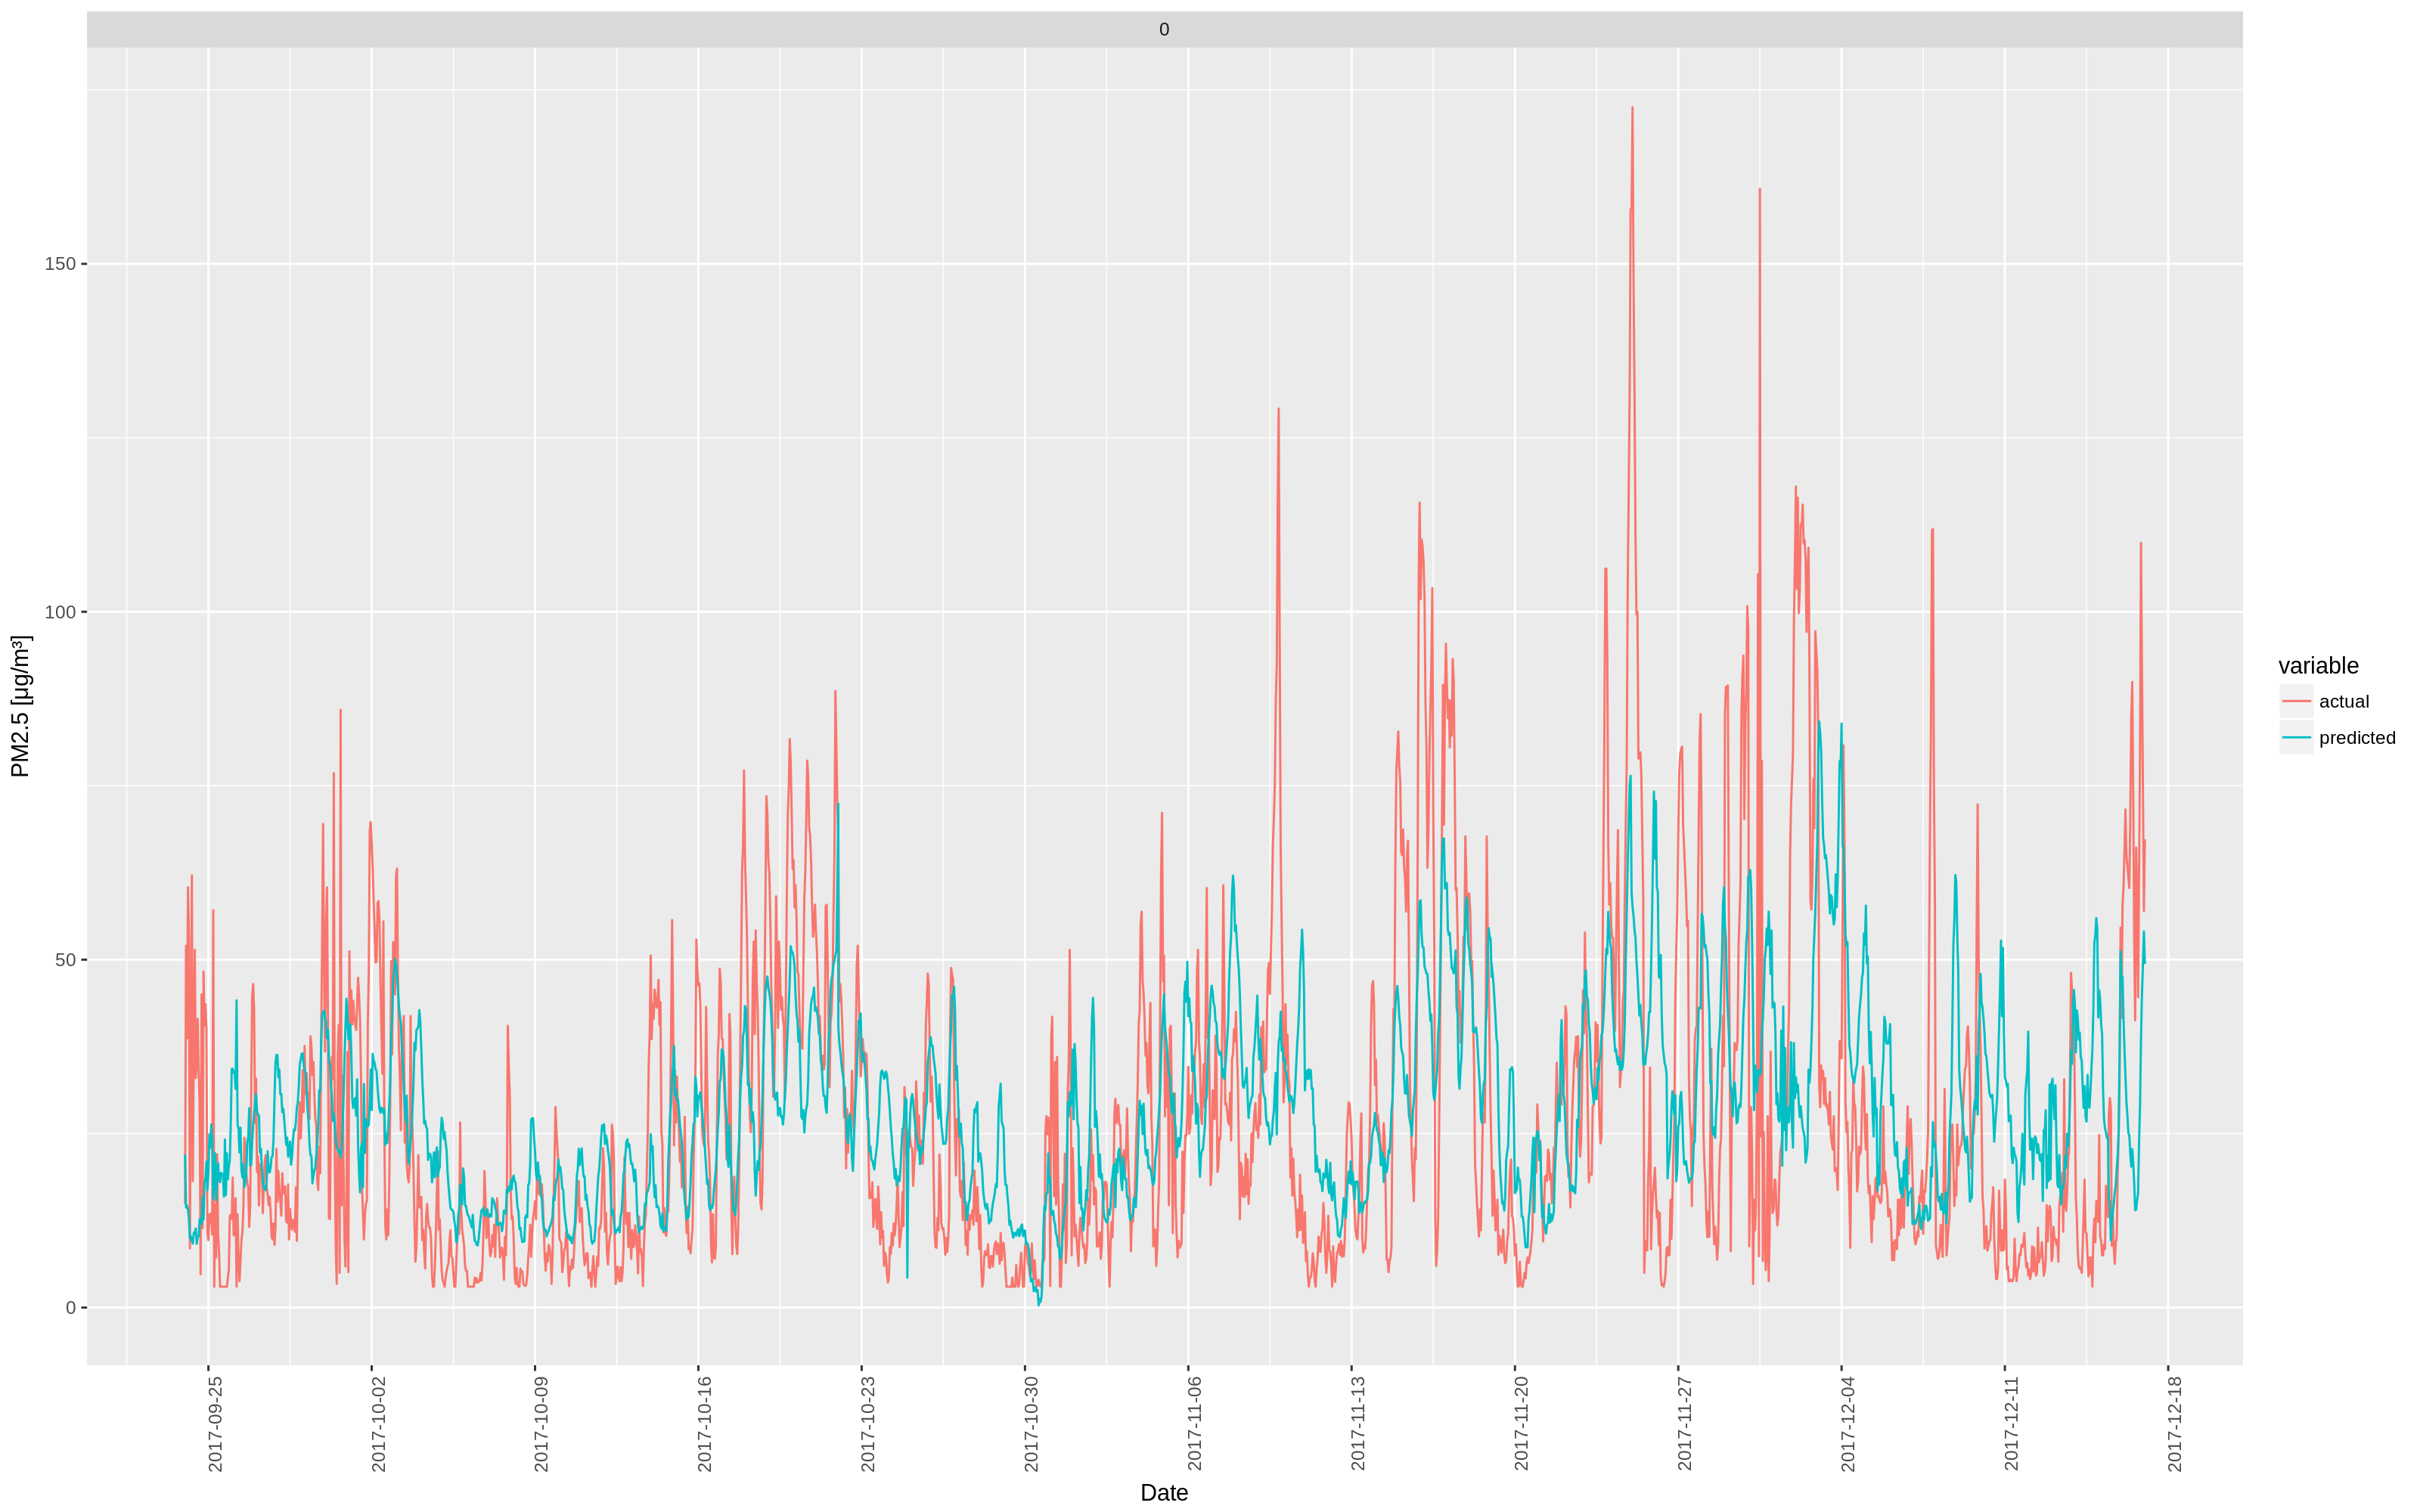
\includegraphics[width=\linewidth]{{figures/results/best-models/bujaka/all-data/autumn/comparison_plot_mlp5_5_5_th_0.5_lag_24}.png}
% \caption{Comparison of actual and predicted PM2.5 concentrations - GIOŚ Bujaka, autumn, all data }
% \label{fig:results-comparison-bujaka-autumn-all-data}
% \end{figure}
% \end{landscape}

% \begin{landscape}
% \begin{figure}[htp]
% \centering
% 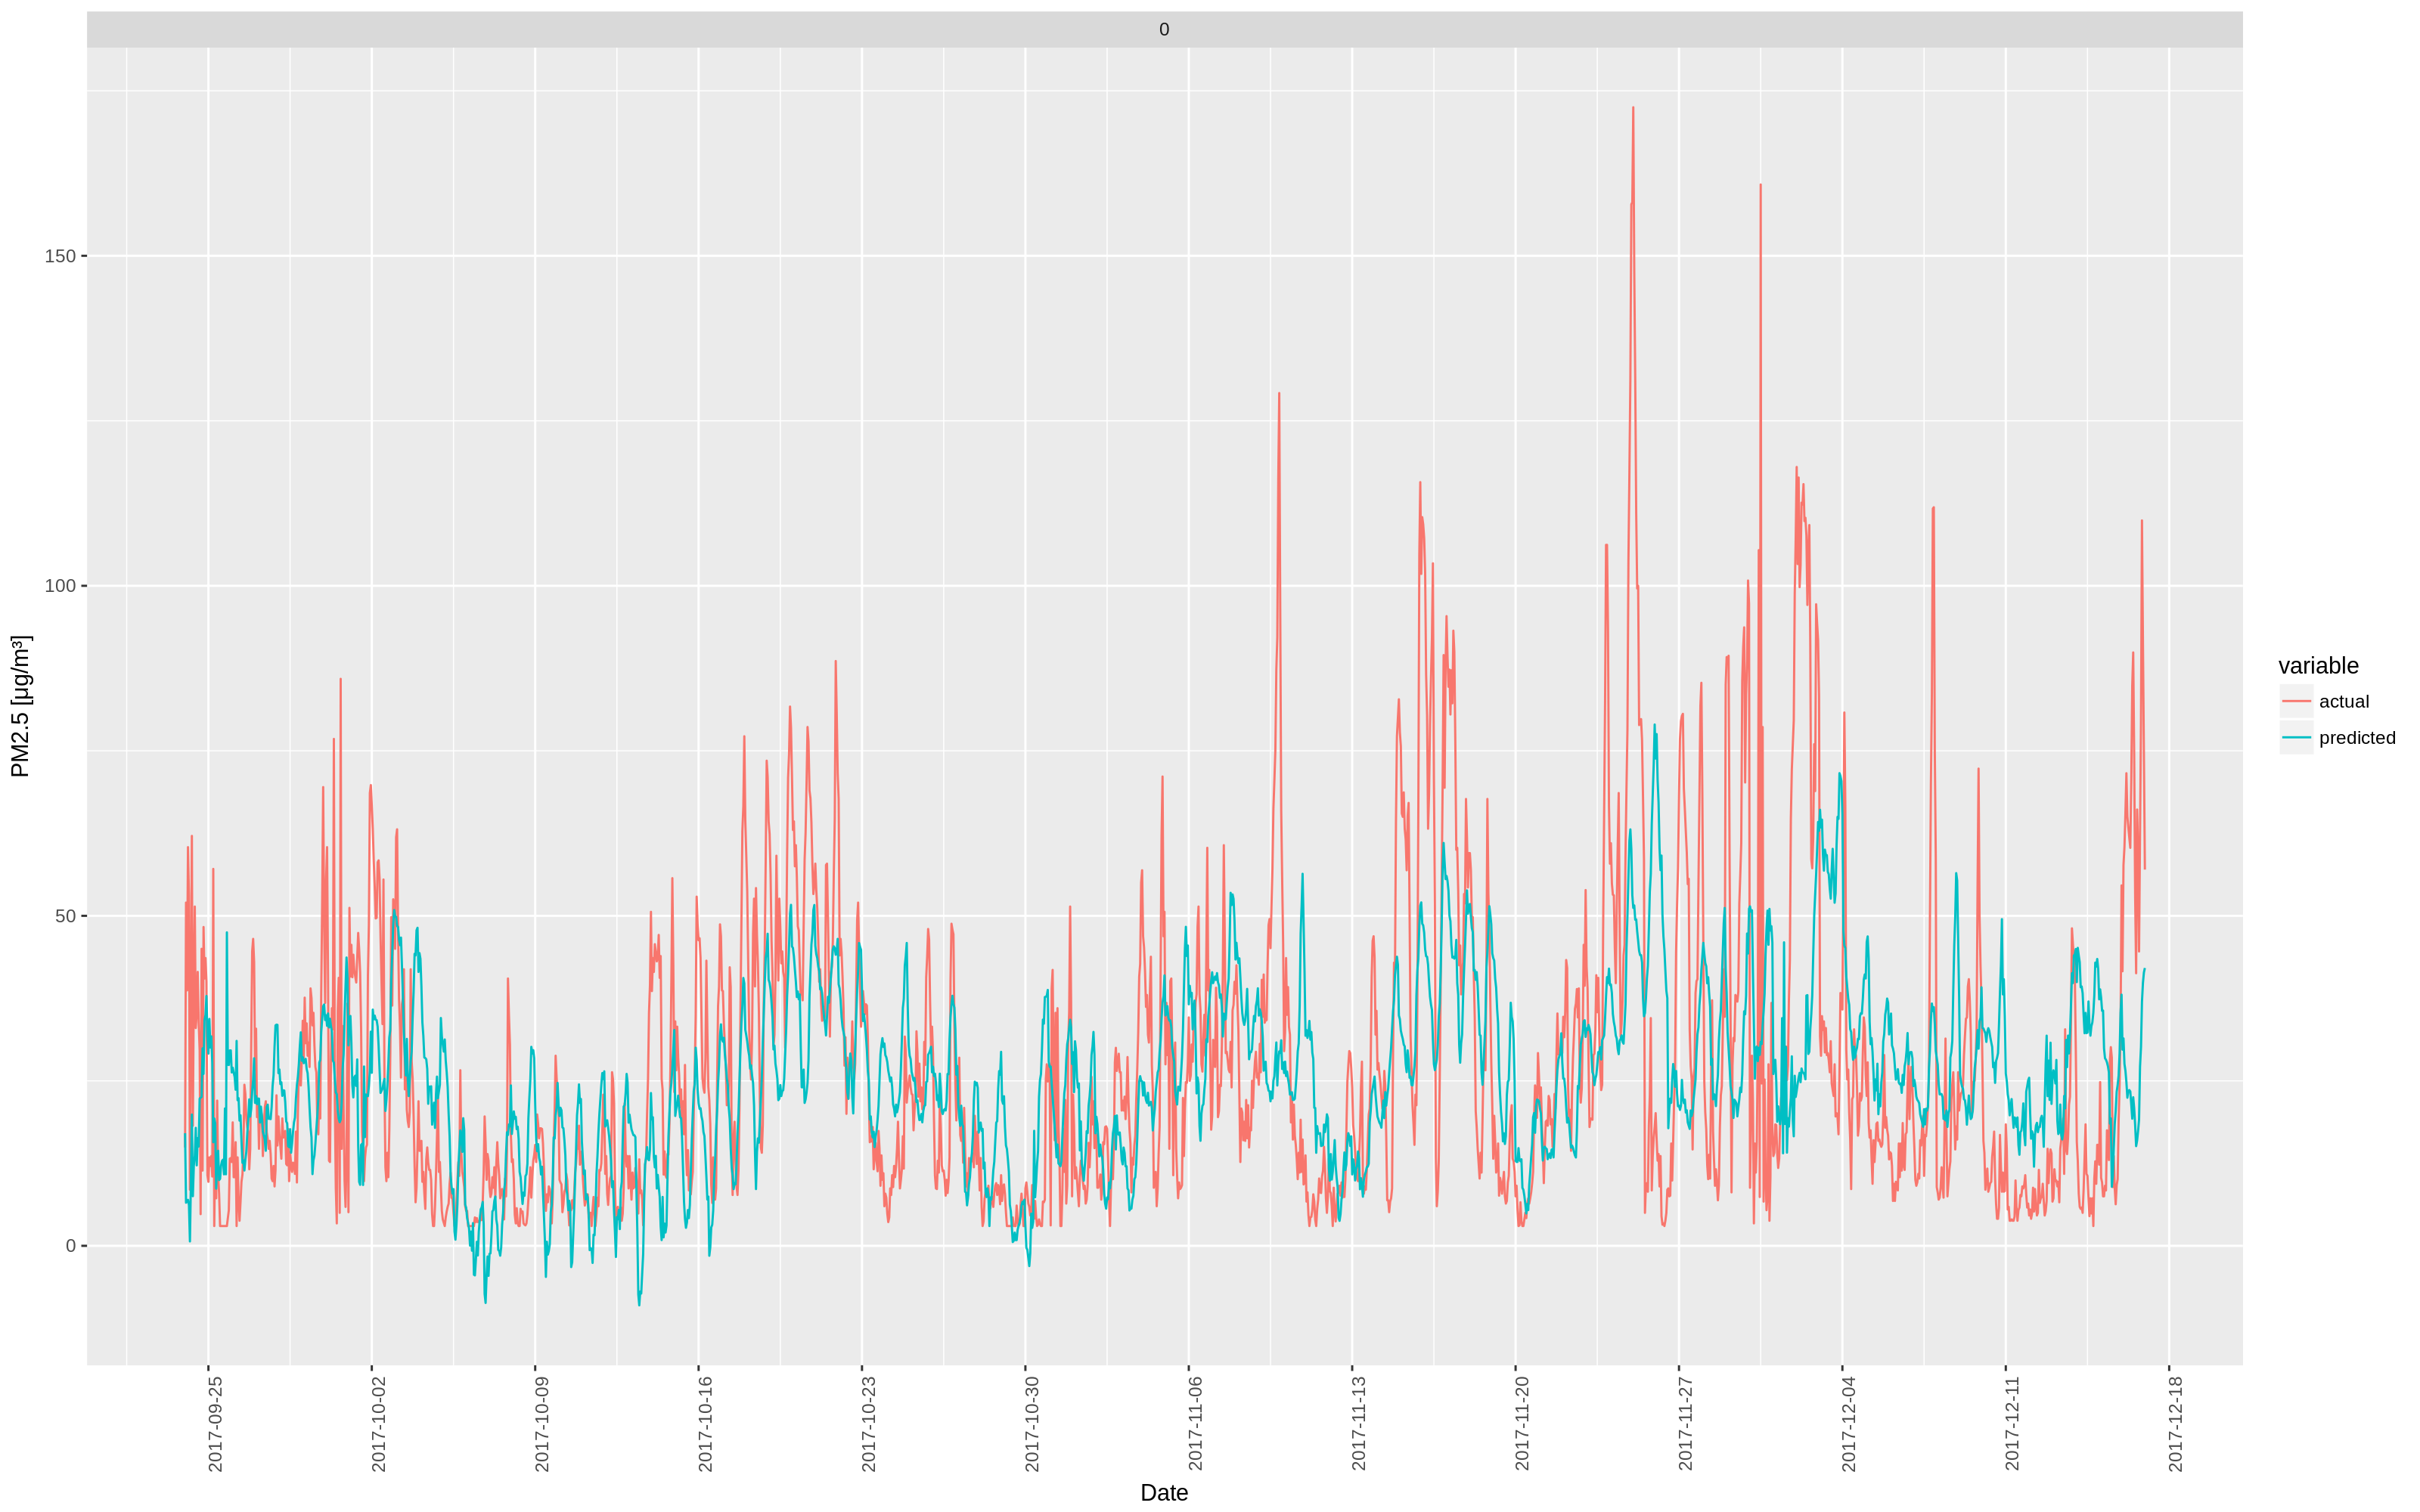
\includegraphics[width=\linewidth]{{figures/results/best-models/bujaka/same-season/autumn/all_comparison_plot_svr_gam0.000244_eps0.5_c16_lag_24}.png}
% \caption{Comparison of actual and predicted PM2.5 concentrations - GIOŚ Bujaka, autumn, same season }
% \label{fig:results-comparison-bujaka-autumn-same-season}
% \end{figure}
% \end{landscape}

% % GIOŚ Bulwarowa

% \begin{landscape}
% \begin{figure}[htp]
% \centering
% \includegraphics[width=\linewidth]{{figures/results/best-models/bulwarowa/all-data/winter/comparison_plot_mlr_lag_24}.png}
% \caption{Comparison of actual and predicted PM2.5 concentrations - GIOŚ Bulwarowa, winter, all data }
% \label{fig:results-comparison-bulwarowa-winter-all-data}
% \end{figure}
% \end{landscape}

% \begin{landscape}
% \begin{figure}[htp]
% \centering
% \includegraphics[width=\linewidth]{{figures/results/best-models/bulwarowa/same-season/winter/all_comparison_plot_lasso_mlr_lag_24}.png}
% \caption{Comparison of actual and predicted PM2.5 concentrations - GIOŚ Bulwarowa, winter, same season }
% \label{fig:results-comparison-bulwarowa-winter-same-season}
% \end{figure}
% \end{landscape}

% \begin{landscape}
% \begin{figure}[htp]
% \centering
% 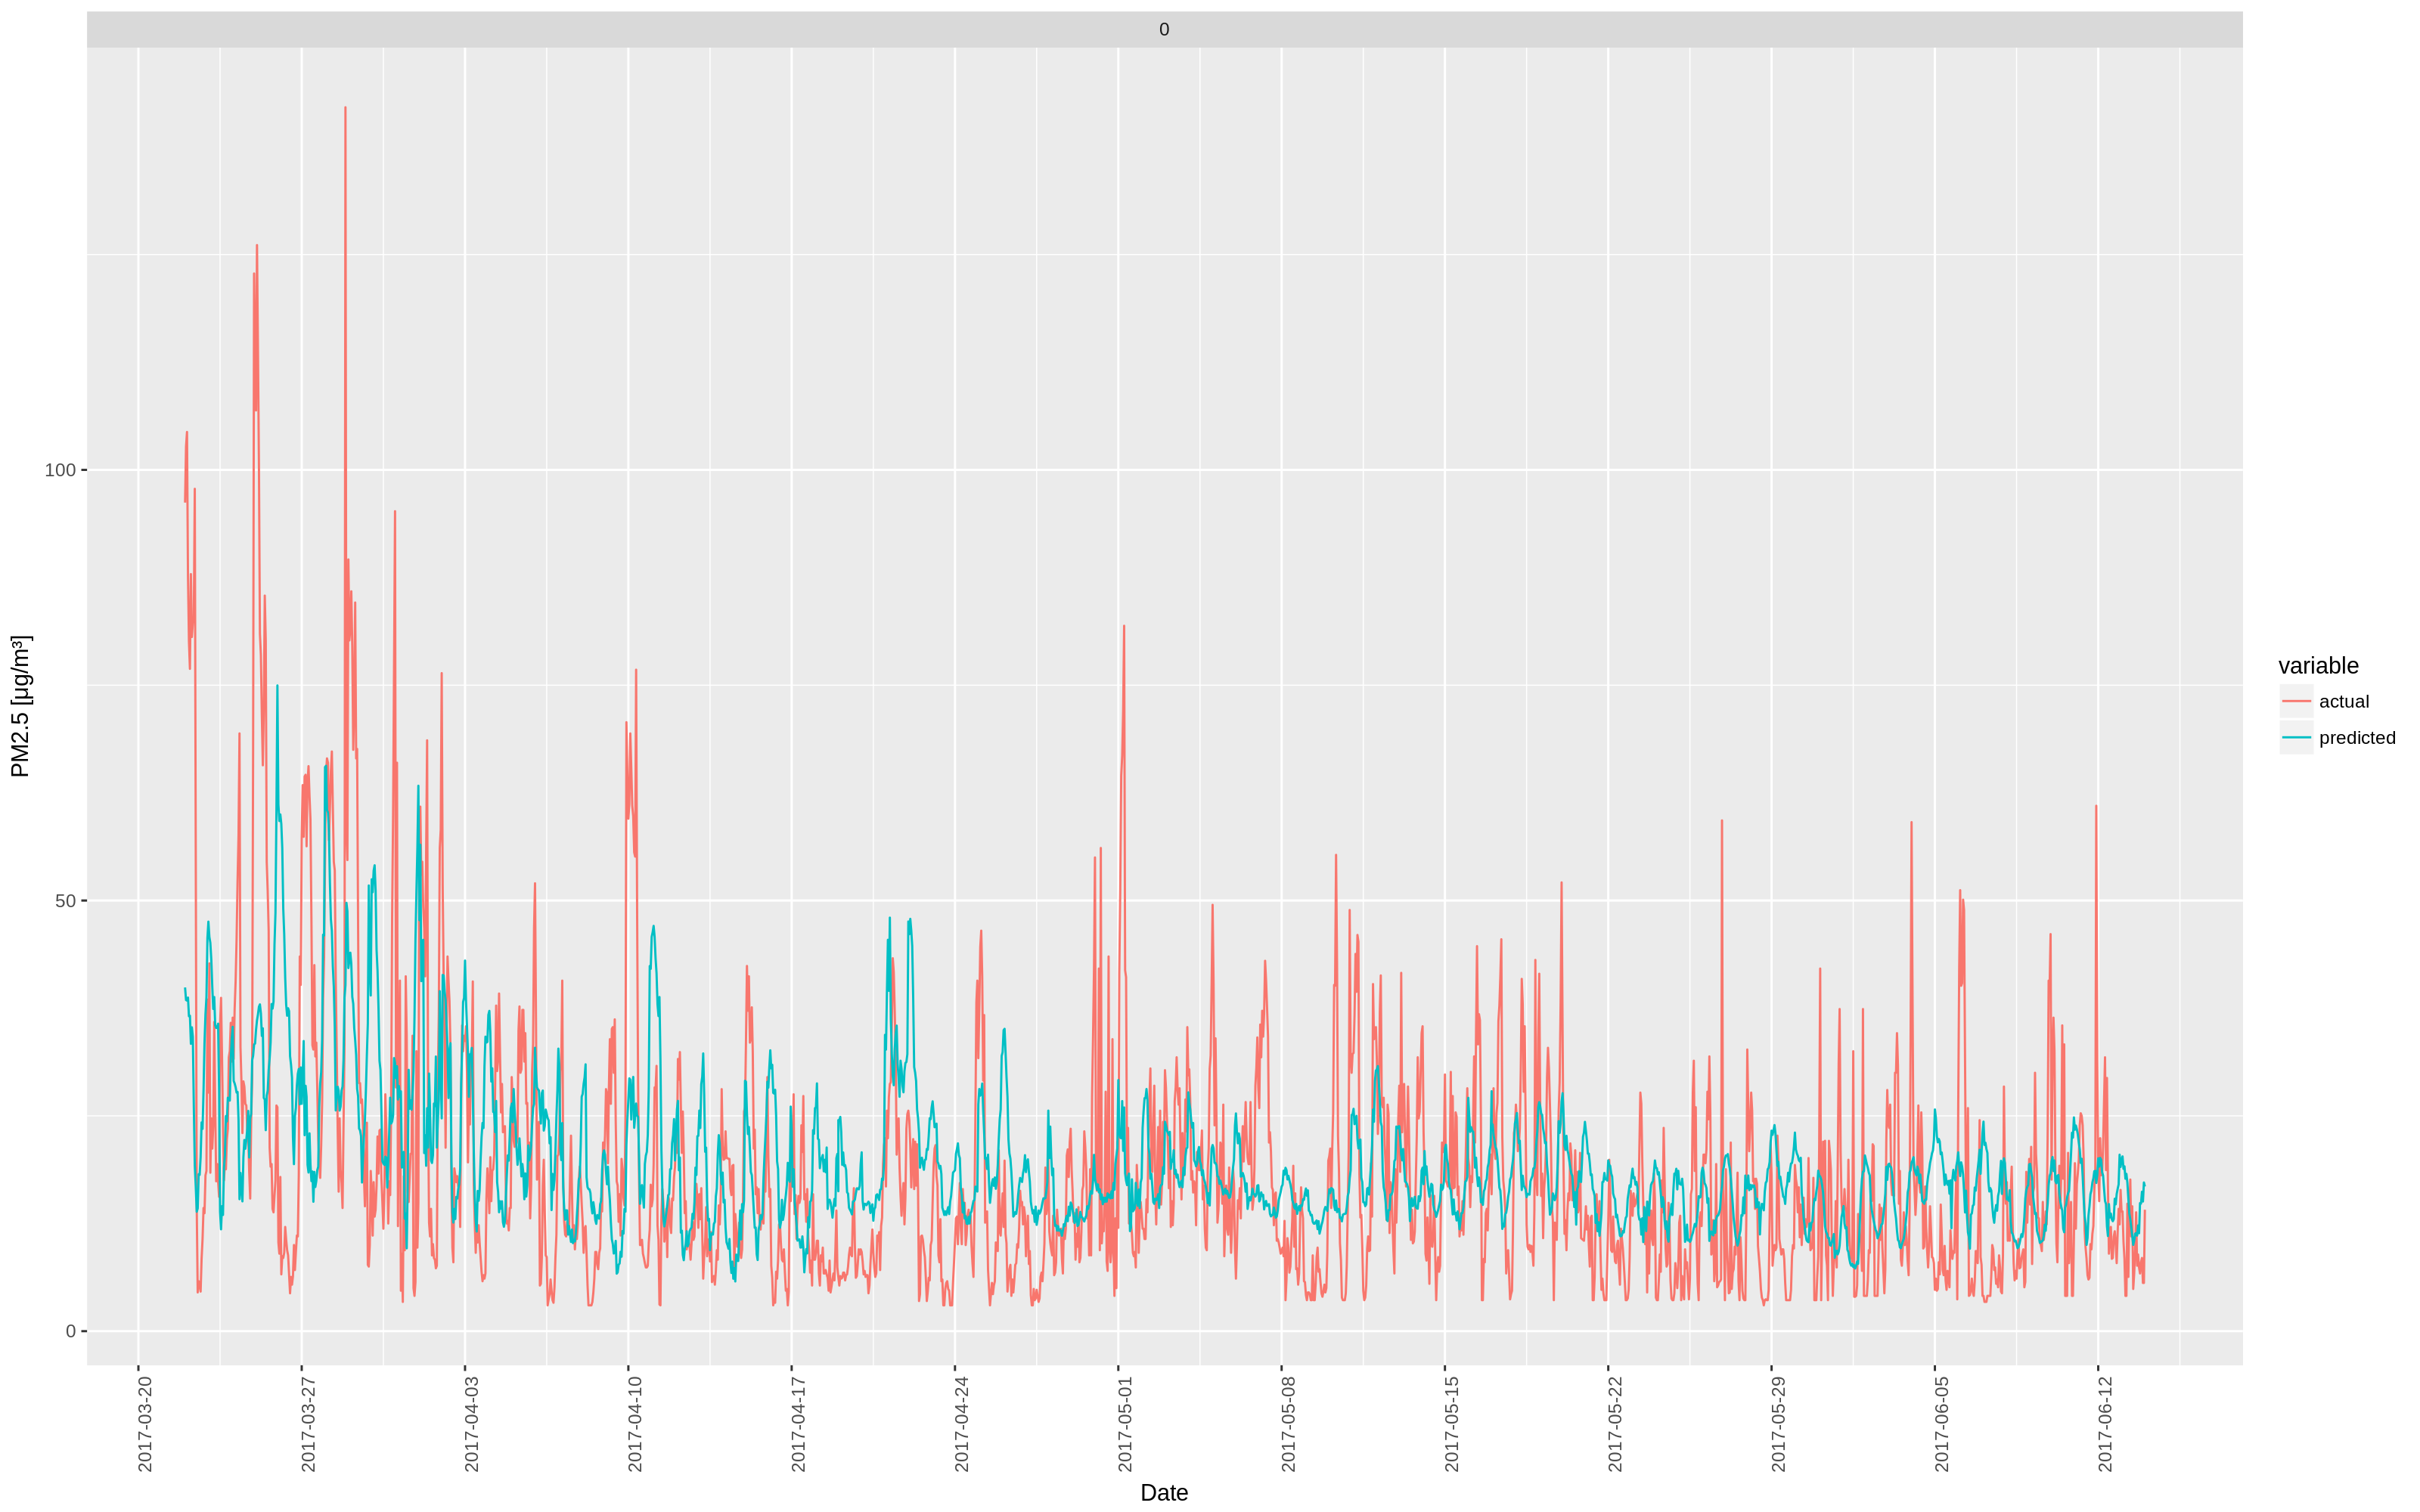
\includegraphics[width=\linewidth]{{figures/results/best-models/bulwarowa/all-data/spring/comparison_plot_mlp3_6_5_th_0.7_lag_24}.png}
% \caption{Comparison of actual and predicted PM2.5 concentrations - GIOŚ Bulwarowa, spring, all data }
% \label{fig:results-comparison-bulwarowa-spring-all-data}
% \end{figure}
% \end{landscape}

% \begin{landscape}
% \begin{figure}[htp]
% \centering
% \includegraphics[width=\linewidth]{{figures/results/best-models/bulwarowa/same-season/spring/all_comparison_plot_svr_gam0.000977_eps0.25_c0.25_lag_24}.png}
% \caption{Comparison of actual and predicted PM2.5 concentrations - GIOŚ Bulwarowa, spring, same season }
% \label{fig:results-comparison-bulwarowa-spring-same-season}
% \end{figure}
% \end{landscape}

% \begin{landscape}
% \begin{figure}[htp]
% \centering
% \includegraphics[width=\linewidth]{{figures/results/best-models/bulwarowa/all-data/summer/comparison_plot_svr_gam0.00391_eps0.0312_c0.25_lag_24}.png}
% \caption{Comparison of actual and predicted PM2.5 concentrations - GIOŚ Bulwarowa, summer, all data }
% \label{fig:results-comparison-bulwarowa-summer-all-data}
% \end{figure}
% \end{landscape}

% \begin{landscape}
% \begin{figure}[htp]
% \centering
% \includegraphics[width=\linewidth]{{figures/results/best-models/bulwarowa/same-season/summer/all_comparison_plot_svr_gam0.000977_eps0.25_c0.25_lag_24}.png}
% \caption{Comparison of actual and predicted PM2.5 concentrations - GIOŚ Bulwarowa, spring, same season }
% \label{fig:results-comparison-bulwarowa-summer-same-season}
% \end{figure}
% \end{landscape}

% \begin{landscape}
% \begin{figure}[htp]
% \centering
% \includegraphics[width=\linewidth]{figures/results/best-models/bulwarowa/all-data/autumn/{comparison_plot_svr_gam0_00391_eps0.0312_c0.25_lag_24}.png}
% \caption{Comparison of actual and predicted PM2.5 concentrations - GIOŚ Bulwarowa, autumn, all data}
% \label{fig:results-comparison-bulwarowa-autumn-all-data}
% \end{figure}
% \end{landscape}

% \begin{landscape}
% \begin{figure}[htp]
% \centering
% \includegraphics[width=\linewidth]{{figures/results/best-models/bulwarowa/same-season/autumn/all_comparison_plot_lasso_mlr_lag_24}.png}
% \caption{Comparison of actual and predicted PM2.5 concentrations - GIOŚ Bulwarowa, autumn, same season }
% \label{fig:results-comparison-bulwarowa-autumn-same-season}
% \end{figure}
% \end{landscape}

% % GIOŚ Krasińskiego
\begin{landscape}
\begin{figure}[ht]
\centering
\includegraphics[width=\linewidth]{{figures/results/best-models/krasinskiego/all-data/winter/comparison_plot_mlr_lag_24}.png}
\caption{Comparison of actual and predicted PM2.5 concentrations - GIOŚ Krasińskiego, winter, all data }
\label{fig:results-comparison-krasinskiego-winter-all-data}
\end{figure}
\end{landscape}

% \begin{landscape}
% \begin{figure}[htp]
% \centering
% \includegraphics[width=\linewidth]{{figures/results/best-models/krasinskiego/same-season/winter/all_comparison_plot_mlr_lag_24}.png}
% \caption{Comparison of actual and predicted PM2.5 concentrations - GIOŚ Krasińskiego, winter, same season }
% \label{fig:results-comparison-krasinskiego-winter-same-season}
% \end{figure}
% \end{landscape}

% \begin{landscape}
% \begin{figure}[htp]
% \centering
% 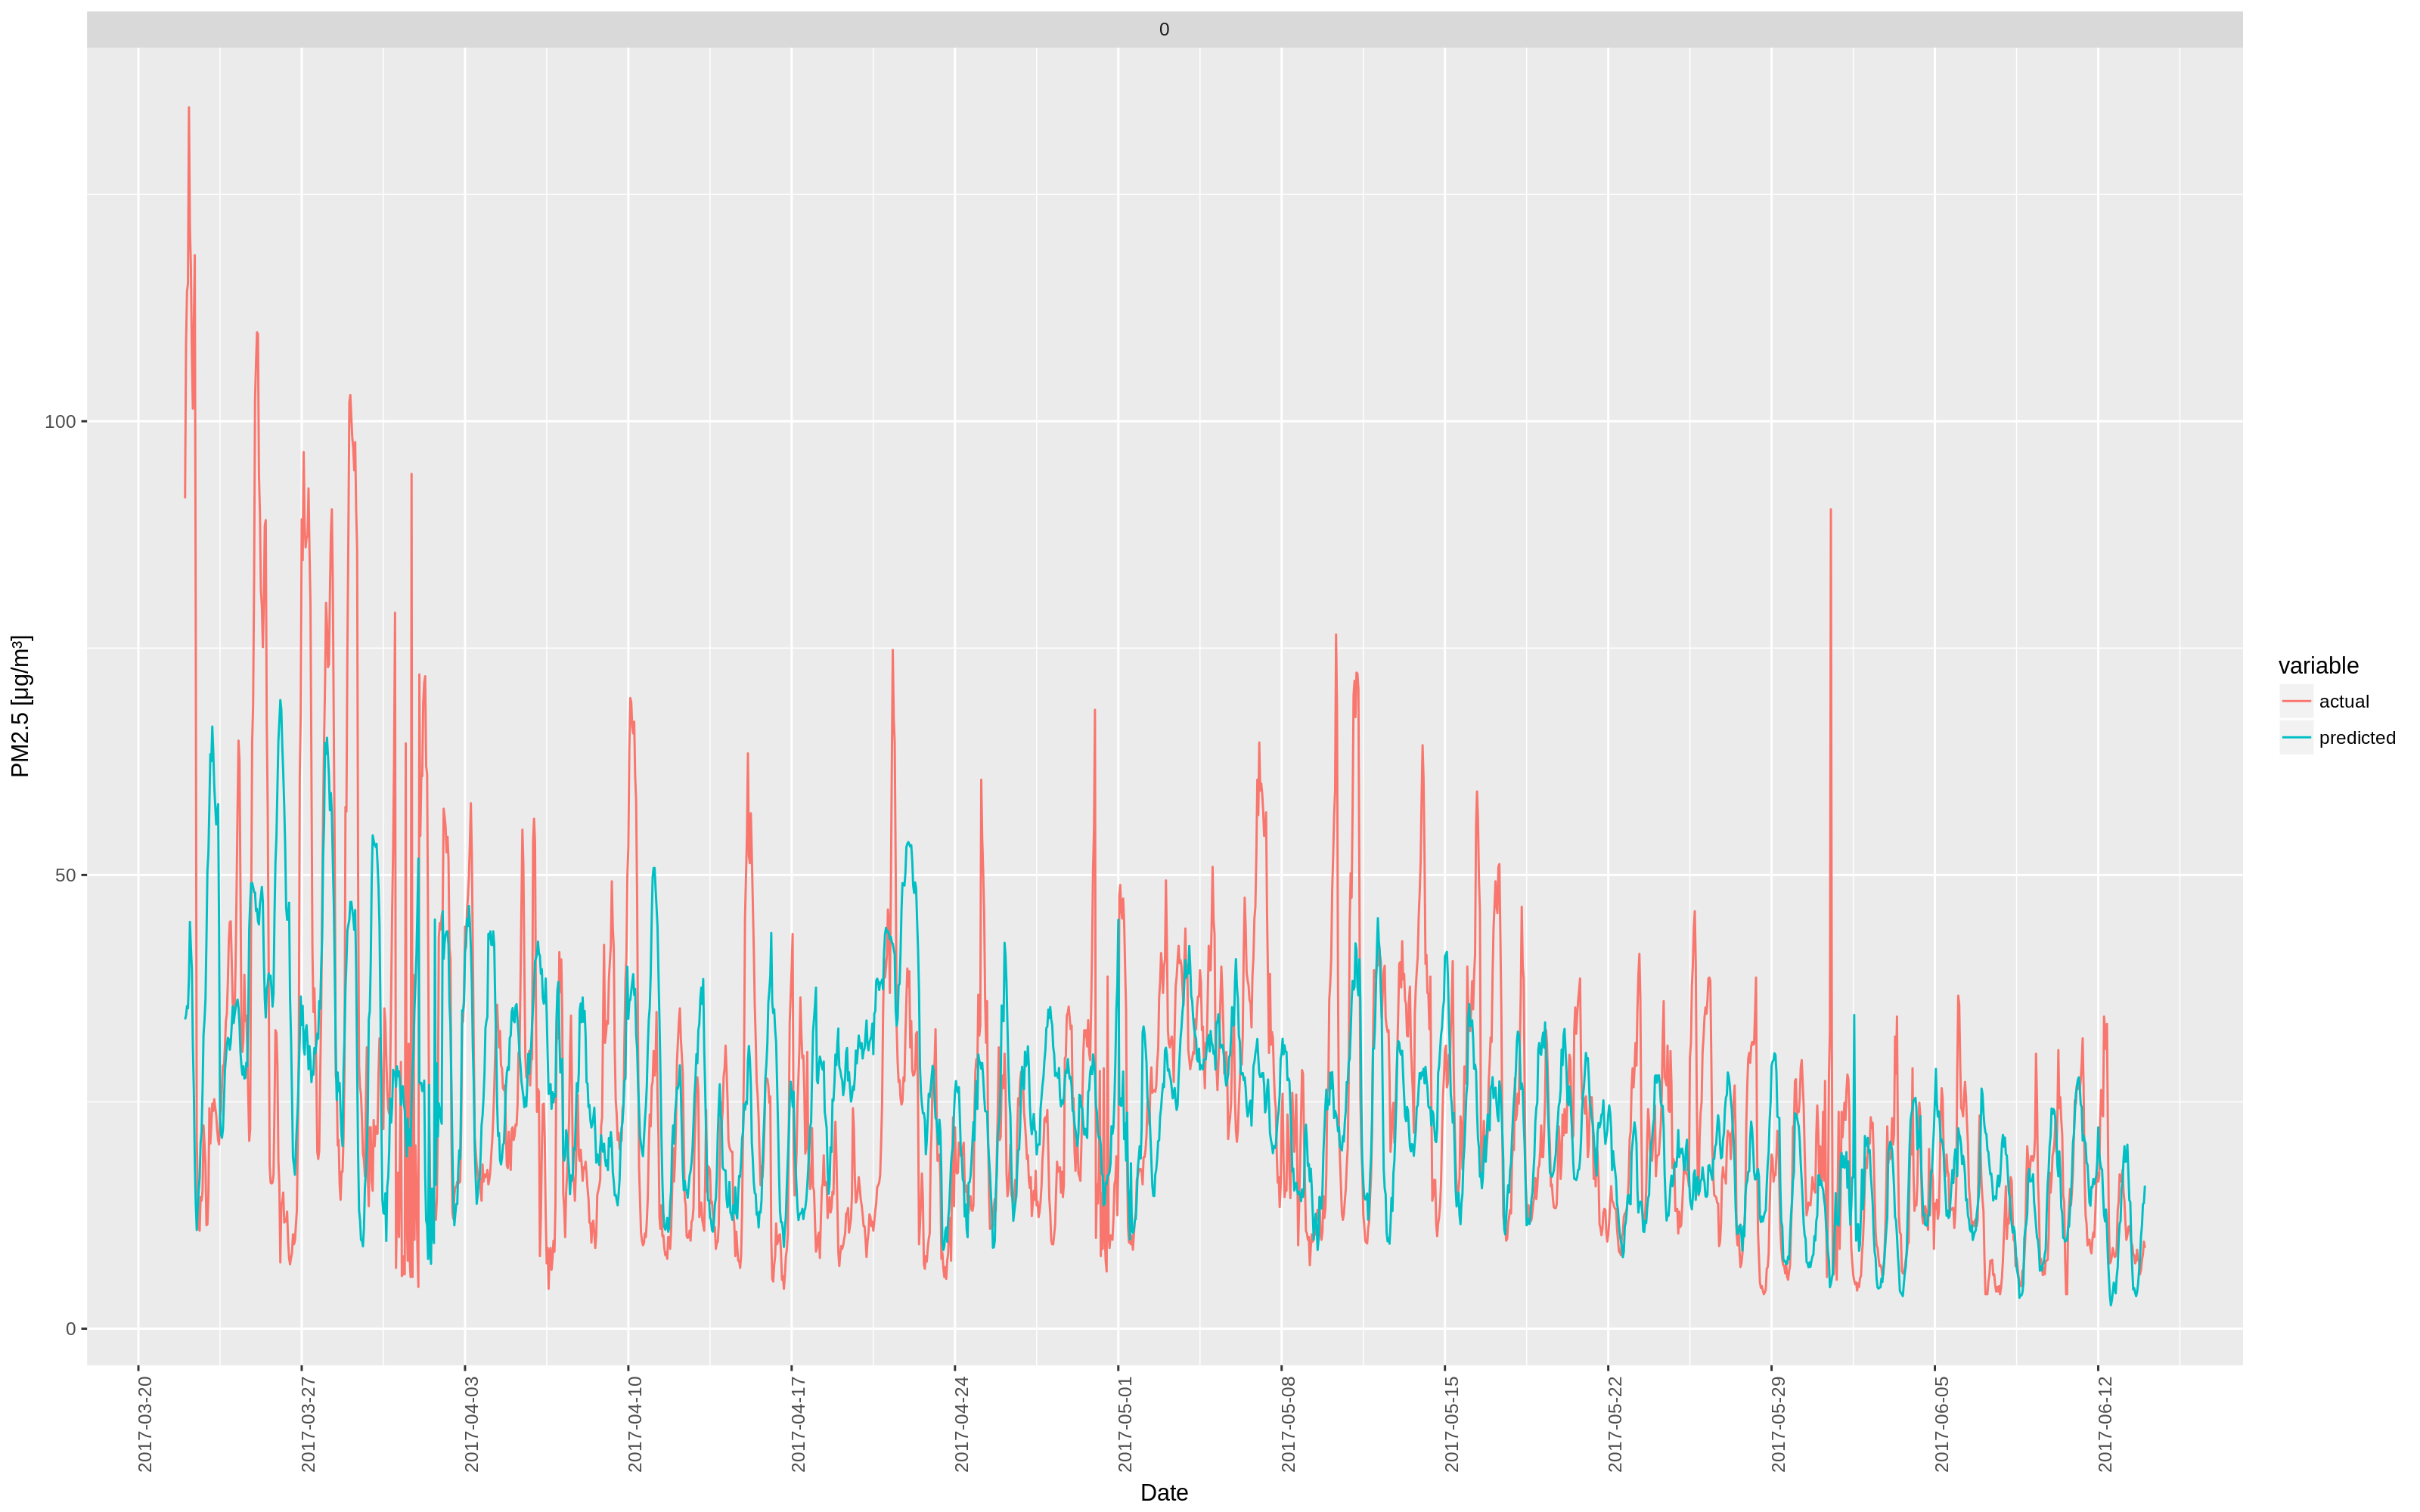
\includegraphics[width=\linewidth]{{figures/results/best-models/krasinskiego/all-data/spring/comparison_plot_svr_gam0.000977_eps2_c1_lag_24}.png}
% \caption{Comparison of actual and predicted PM2.5 concentrations - GIOŚ Krasińskiego, spring, all data }
% \label{fig:results-comparison-krasinskiego-spring-all-data}
% \end{figure}
% \end{landscape}

% \begin{landscape}
% \begin{figure}[htp]
% \centering
% \includegraphics[width=\linewidth]{{figures/results/best-models/krasinskiego/same-season/spring/all_comparison_plot_svr_gam0.000977_eps0.25_c0.25_lag_24}.png}
% \caption{Comparison of actual and predicted PM2.5 concentrations - GIOŚ Krasińskiego, spring, same season }
% \label{fig:results-comparison-krasinskiego-spring-same-season}
% \end{figure}
% \end{landscape}

% \begin{landscape}
% \begin{figure}[htp]
% \centering
% \includegraphics[width=\linewidth]{{figures/results/best-models/krasinskiego/all-data/summer/comparison_plot_svr_gam0.00391_eps0.0312_c0.25_lag_24}.png}
% \caption{Comparison of actual and predicted PM2.5 concentrations - GIOŚ Krasińskiego, summer, all data }
% \label{fig:results-comparison-krasinskiego-summer-all-data}
% \end{figure}
% \end{landscape}

% \begin{landscape}
% \begin{figure}[htp]
% \centering
% 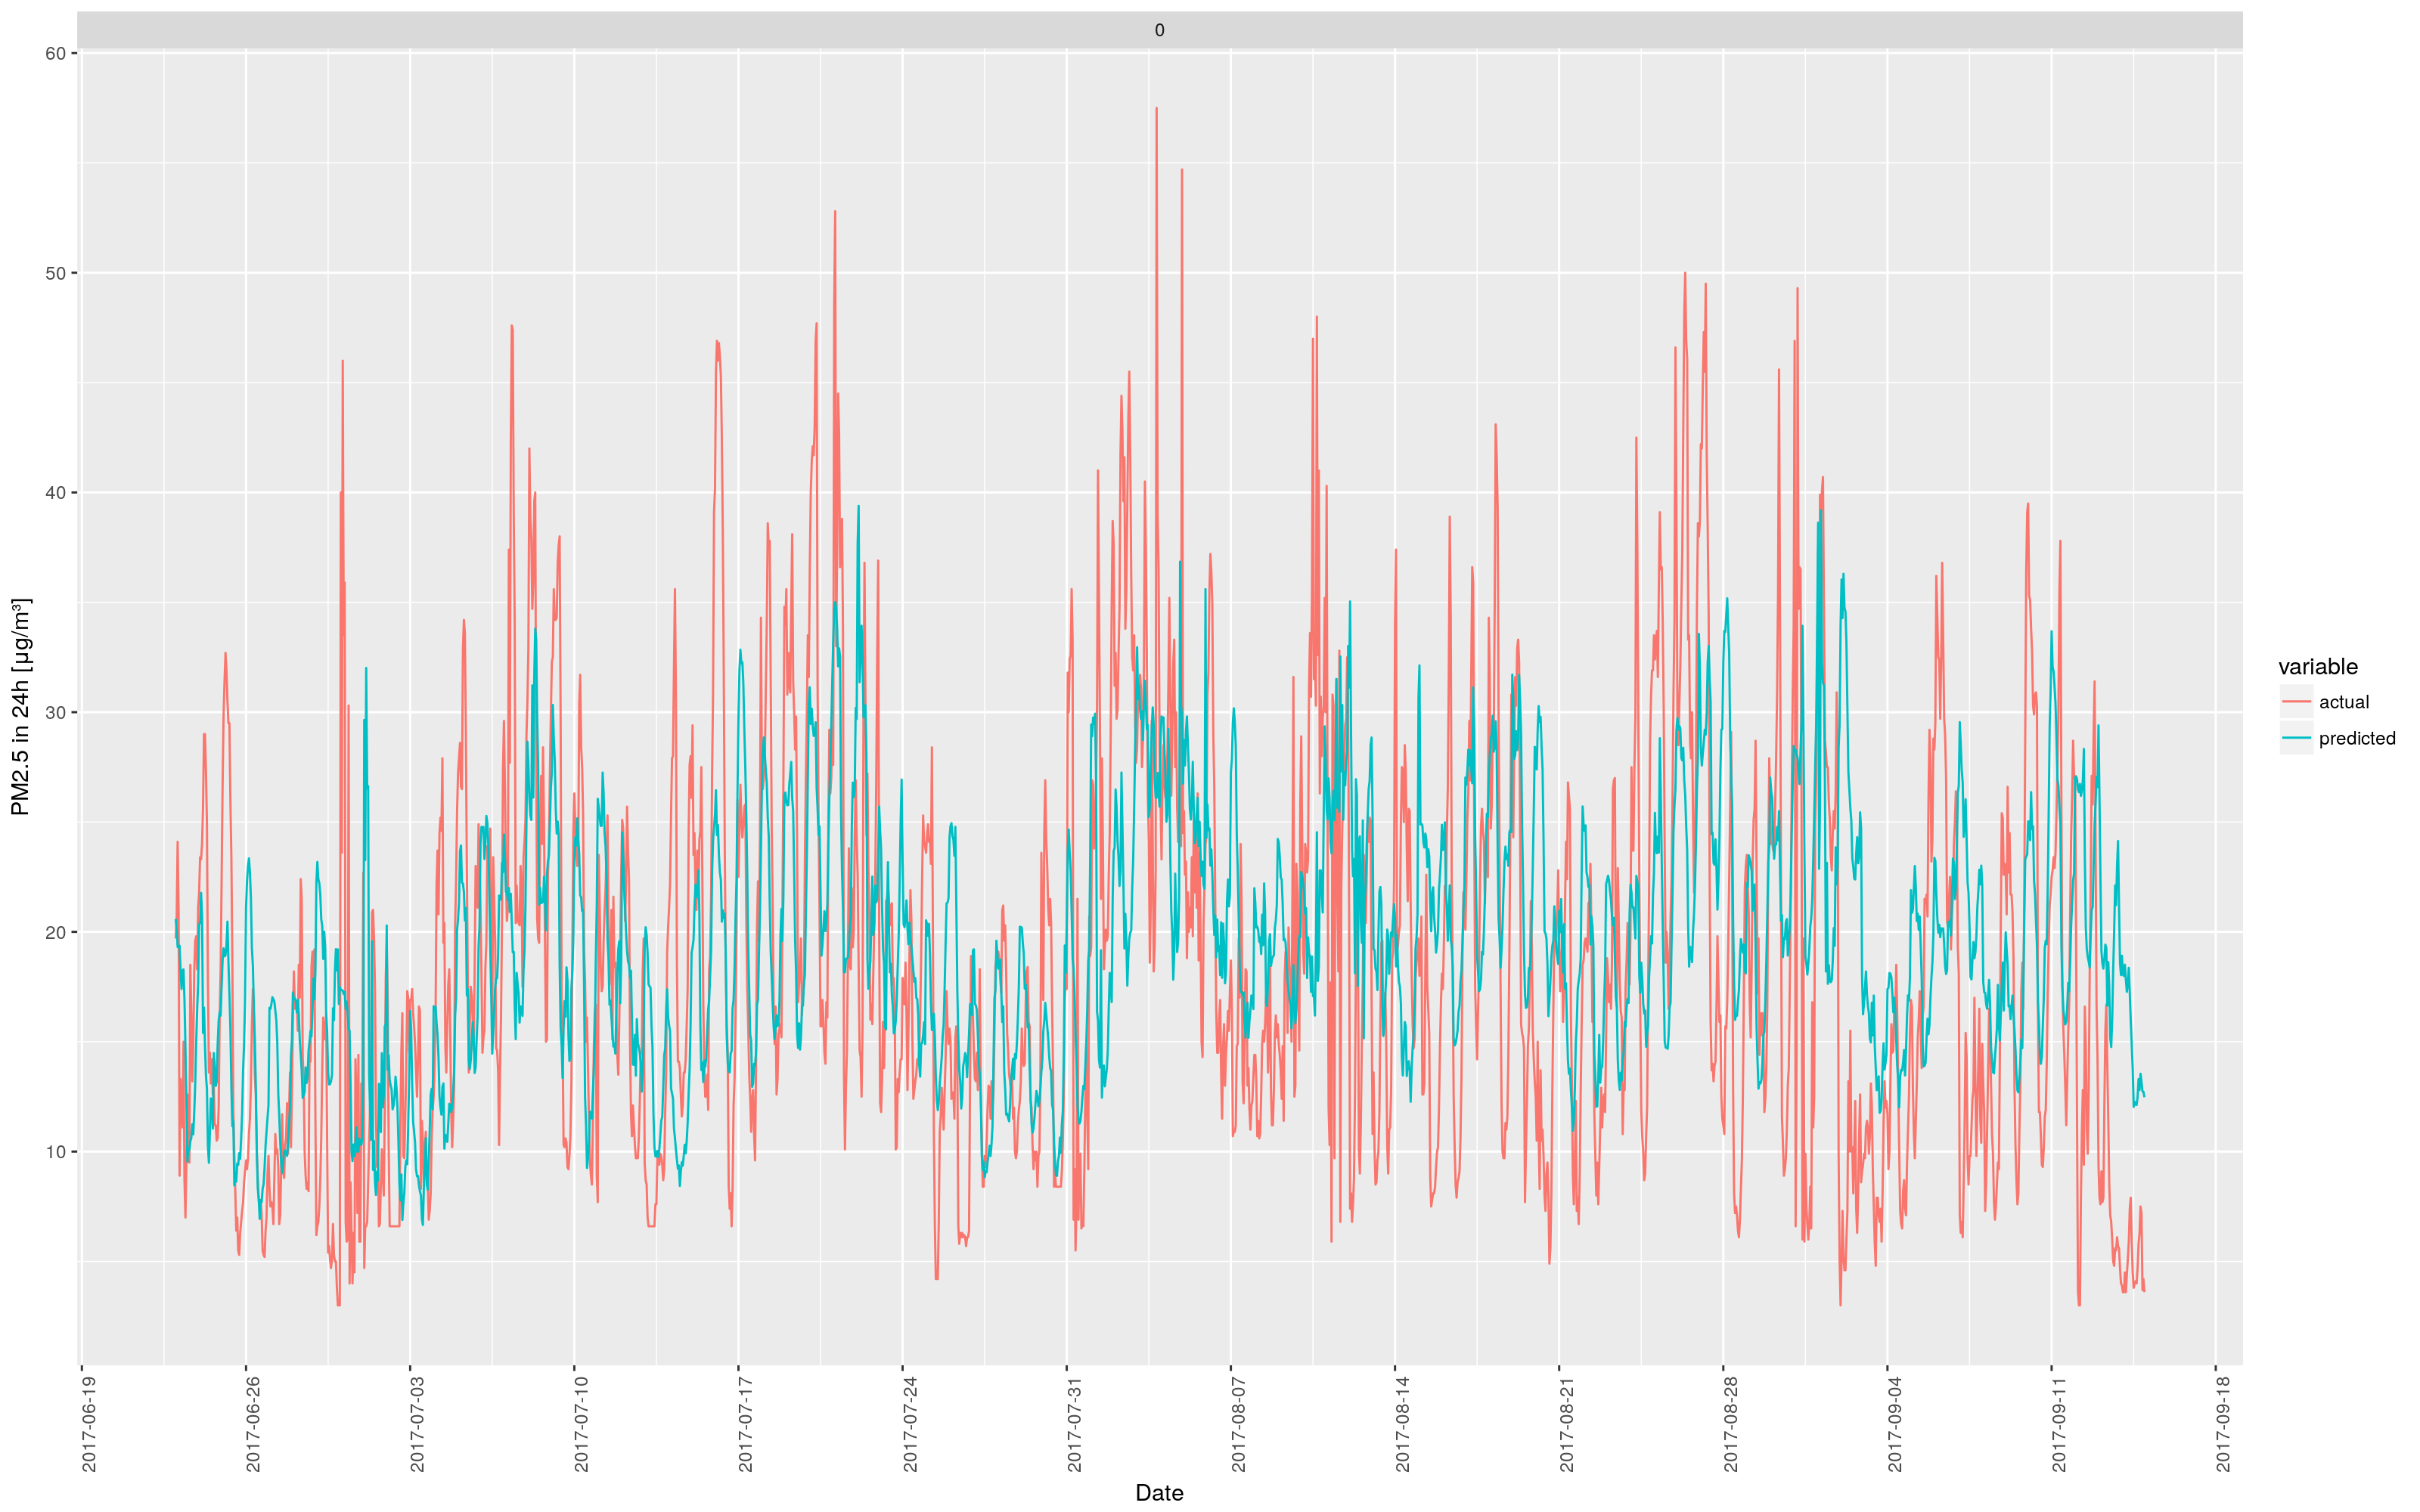
\includegraphics[width=\linewidth]{{figures/results/best-models/krasinskiego/same-season/summer/all_comparison_plot_lasso3_lag_24}.png}
% \caption{Comparison of actual and predicted PM2.5 concentrations - GIOŚ Krasińskiego, spring, same season }
% \label{fig:results-comparison-krasinskiego-summer-same-season}
% \end{figure}
% \end{landscape}

% \begin{landscape}
% \begin{figure}[htp]
% \centering
% 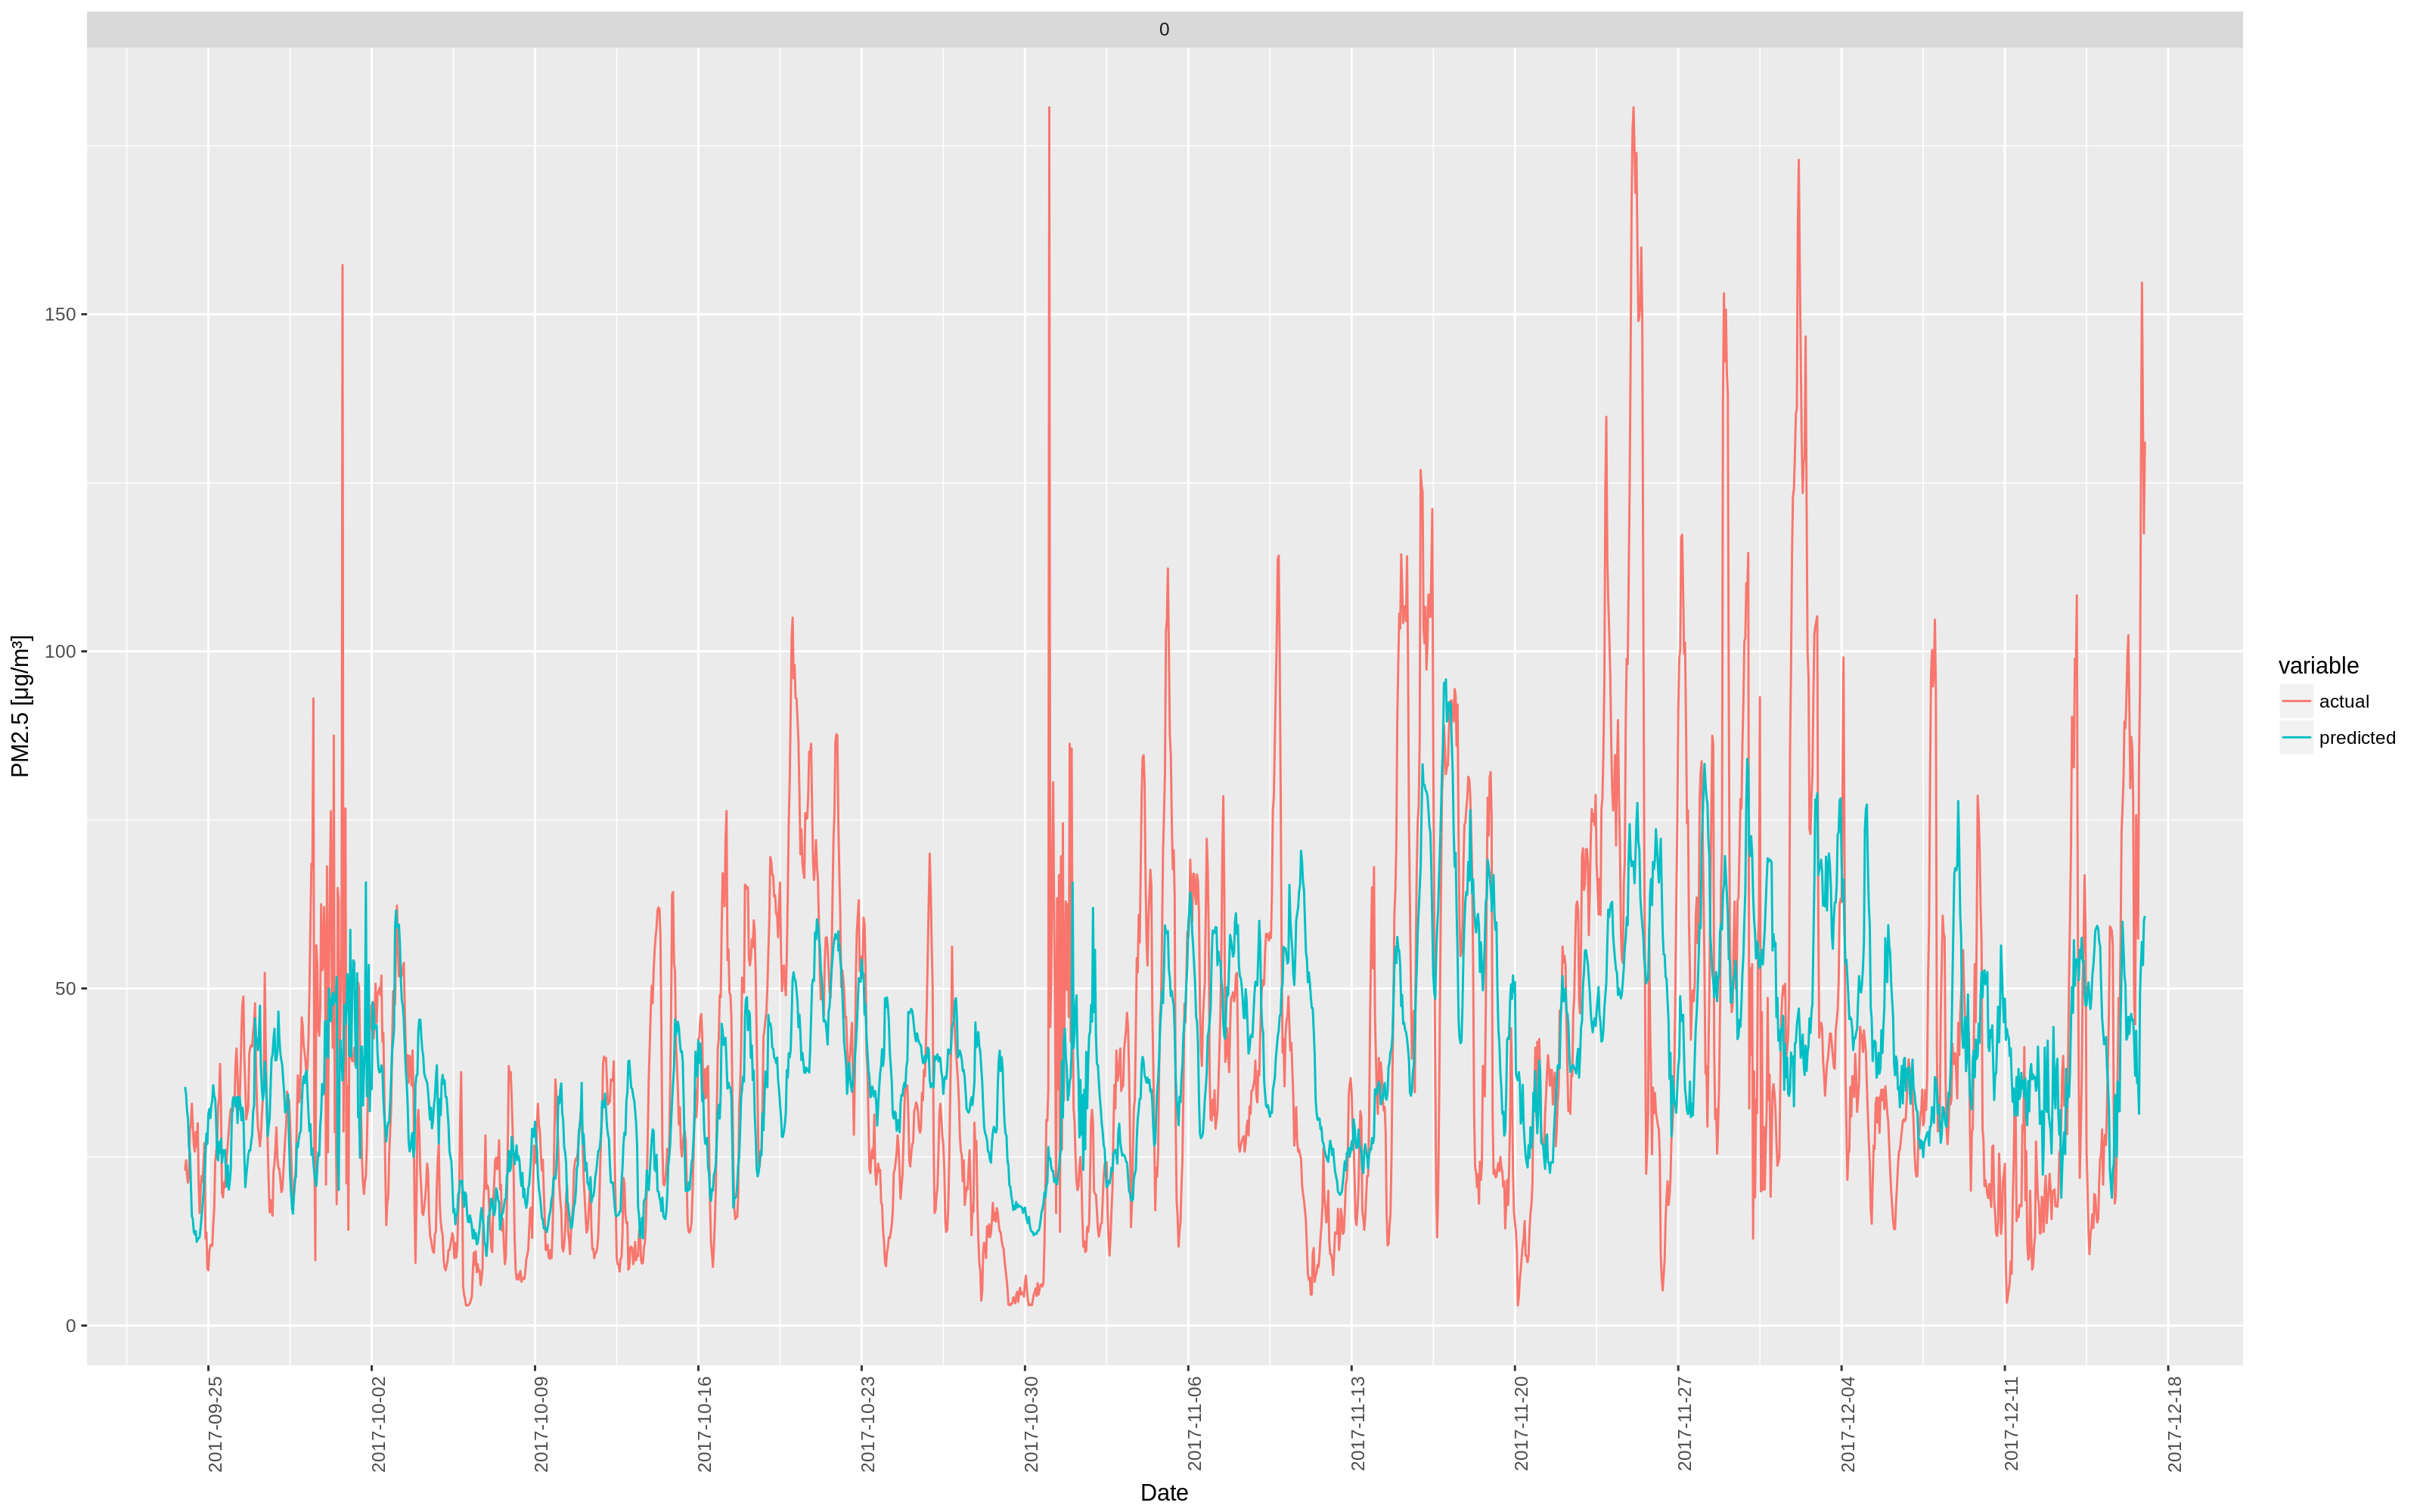
\includegraphics[width=\linewidth]{{figures/results/best-models/krasinskiego/all-data/autumn/comparison_plot_mlp2_5_5_th_0.5_lag_24}.png}
% \caption{Comparison of actual and predicted PM2.5 concentrations - GIOŚ Krasińskiego, autumn, all data }
% \label{fig:results-comparison-krasinskiego-autumn-all-data}
% \end{figure}
% \end{landscape}

% \begin{landscape}
% \begin{figure}[htp]
% \centering
% 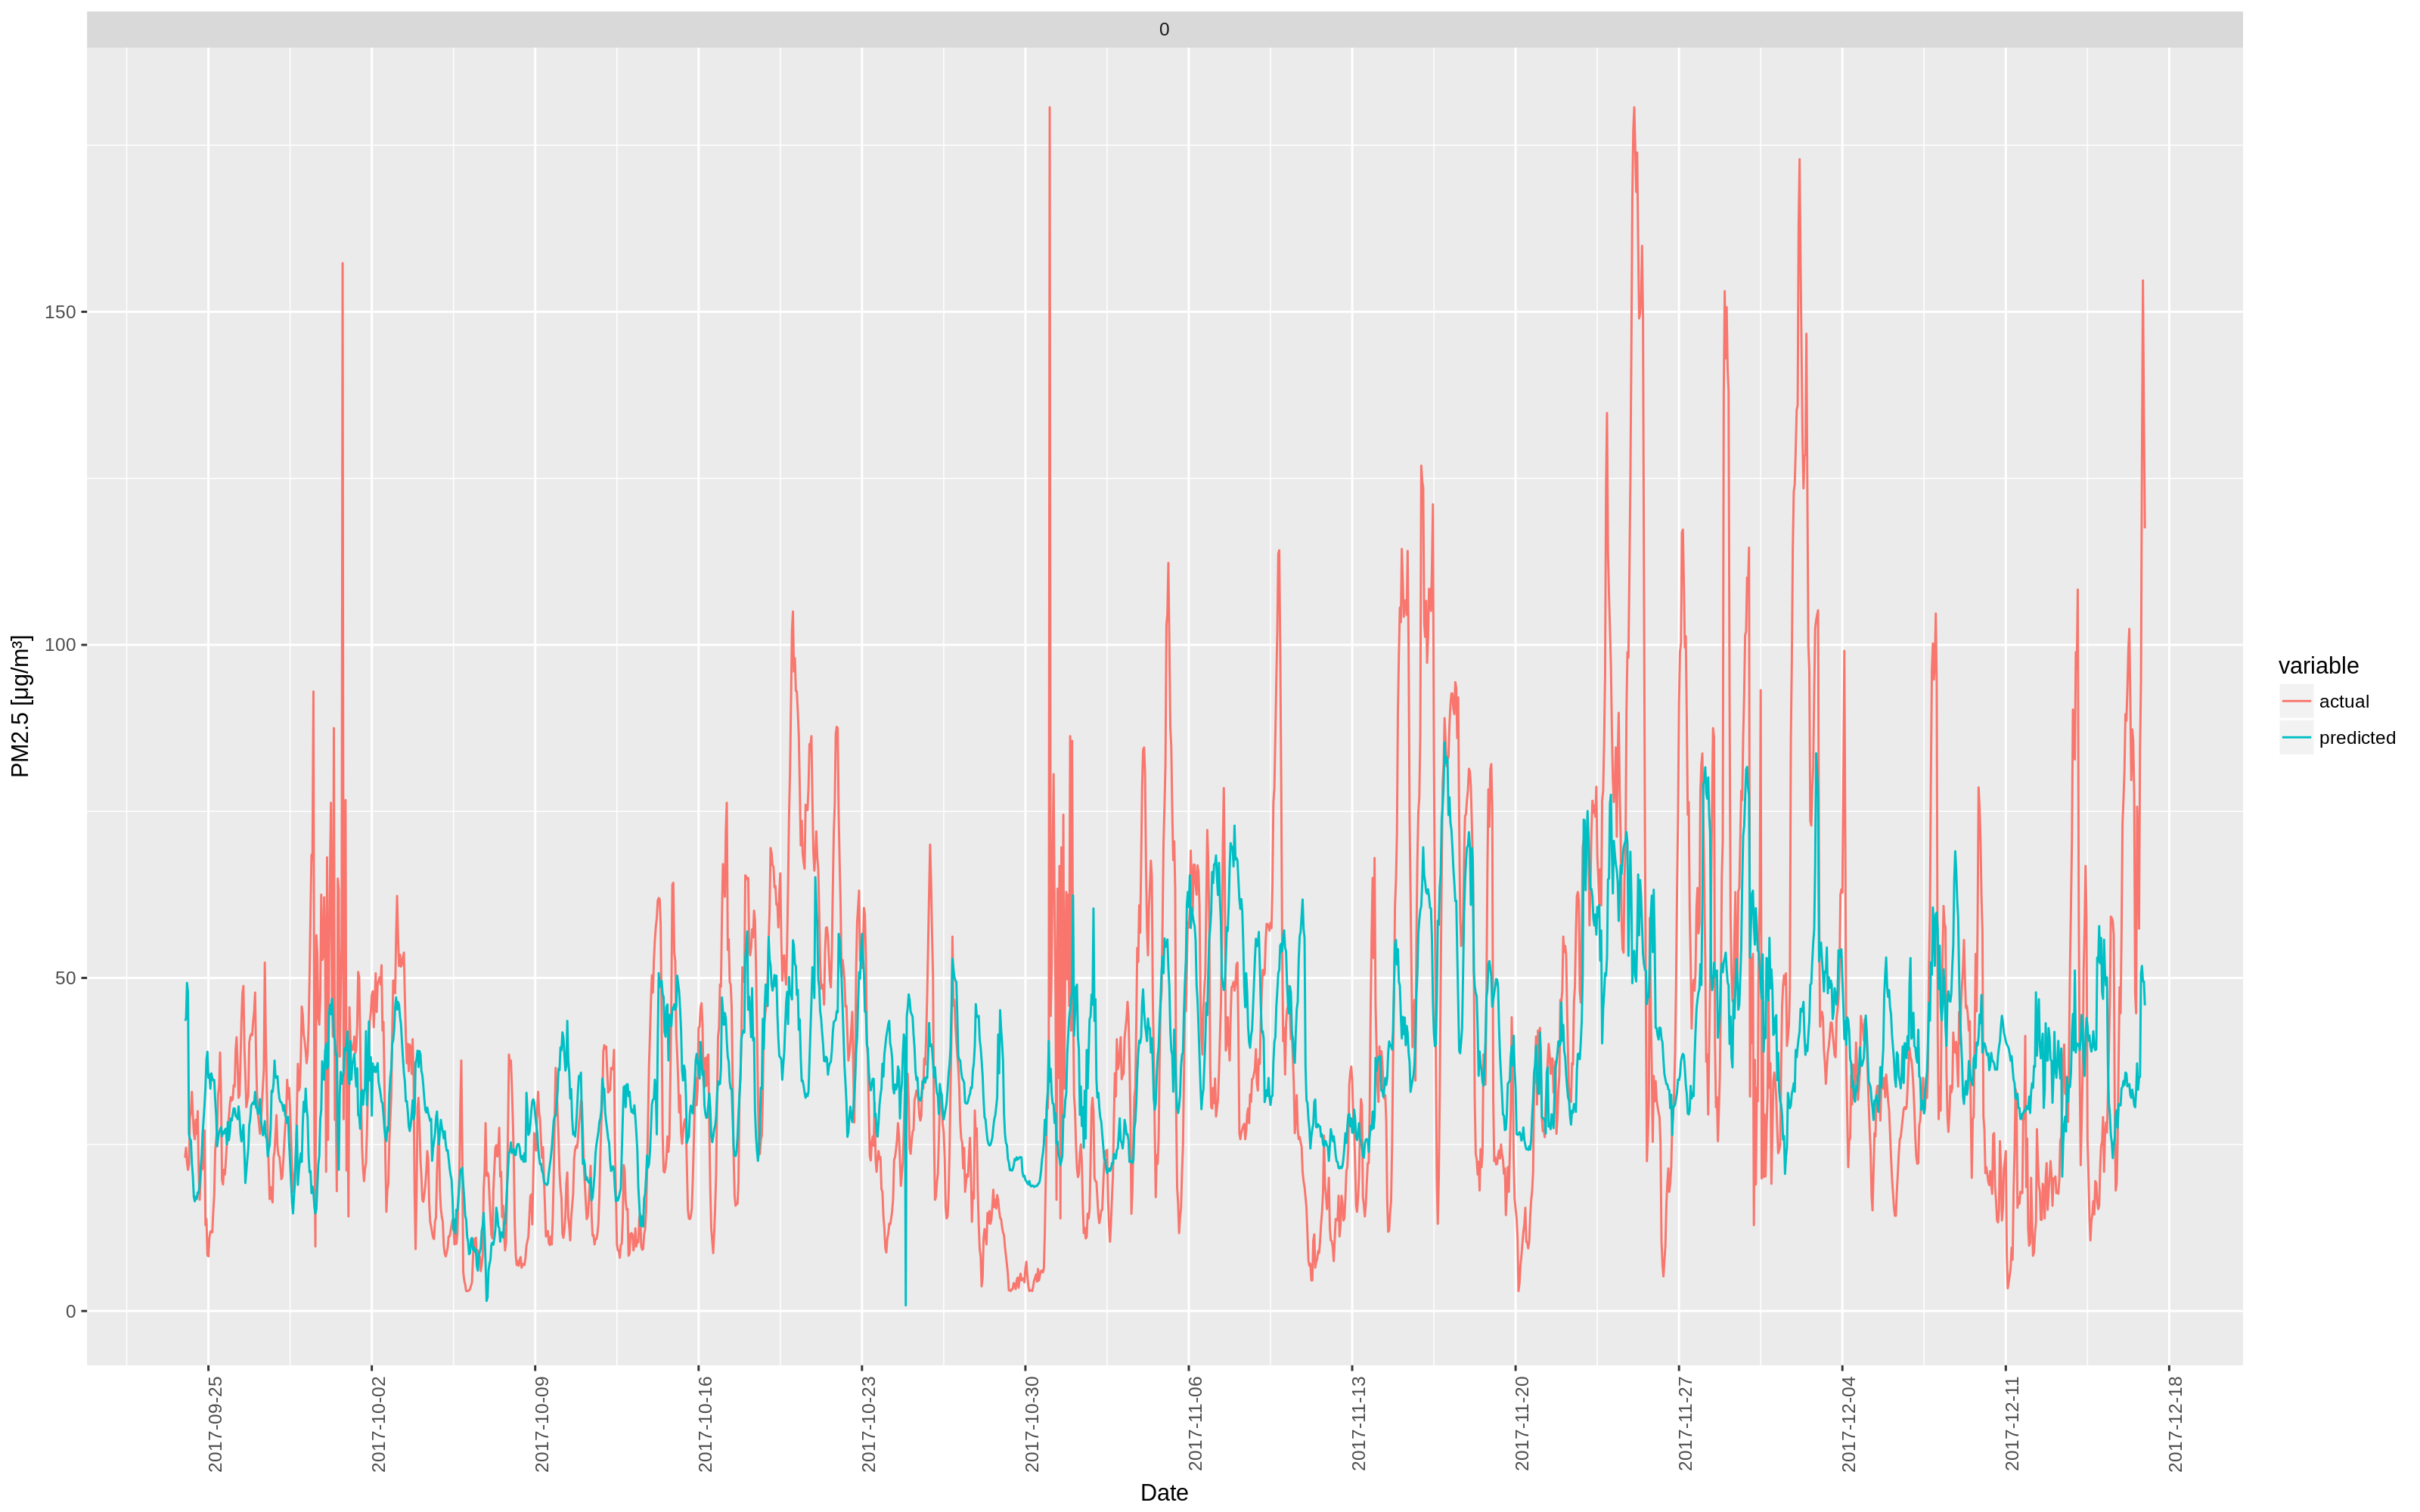
\includegraphics[width=\linewidth]{{figures/results/best-models/krasinskiego/same-season/autumn/all_comparison_plot_mlp4_3_2_th_0.3_lag_24}.png}
% \caption{Comparison of actual and predicted PM2.5 concentrations - GIOŚ Krasińskiego, autumn, same season }
% \label{fig:results-comparison-krasinskiego-autumn-same-season}
% \end{figure}
% \end{landscape}